% This part is the latex header. It defines what kind of document this will be and 
% says which packages to use. Packages let you include different kind of formats
% and templates in the document. 
\documentclass[11pt]{article} % document type - other options are journal or book?
\usepackage[pdftex]{graphicx} % package to import figures
\usepackage{float} % used for placing figures - H
\usepackage{hyperref} % used for including links (hyper links)
\usepackage{enumerate} % used for making lists
\usepackage[margin=1cm]{geometry}
\usepackage{tabularx}
\usepackage{booktabs}
\usepackage{amsmath}
\usepackage[version=3]{mhchem} 
\usepackage{siunitx}

% math packages
\usepackage{amssymb}
\usepackage{amsmath}

\pagestyle{headings}
\topmargin -0.5in
\oddsidemargin 0.0in
\textwidth 6.5in
\textheight 9.0in

% declare the title, date and author
\title{Radial Bias Pilot 1}
\date{Mar 3, 2021}
\author{Rania Ezzo}

% This is where the actual document starts
\begin{document}
\maketitle
\tableofcontents


\section{Goal of Pilot 1}
To measure radial direction bias with 1D drifting gratings at 2-4 polar angle locations at a given eccentricity. A total of 4 directions of motion will be tested, 2 radial (inwards and outwards) and 2 tangential (clockwise, counterclockwise), to measure the performance differences between (1) centrifugal and centripetal motion directions, and (2) radial and tangential motion directions. 

\subsection{Parameters}
Eccentricity from central fixation: 7 degrees
\\
Locations tested (polar angle relative to fixation): Upper left (45 deg) and lower right (225 deg)
\\
Stimulus: sine wave gratings w/ 0.4 deg sigma gaussian mask
\\
Stimulus spatial frequency: 1 c/deg
\\
Stimulus drift speed: 4 deg/s
\\
Stimulus contrast: full contrast + gaussian mask
\\
Stimulus aperature diameter: 2.5 deg
\\
Black circular aperature was put onto screen to avoid perceptual artifacts from screen edges
\\
Number of subjects: 1

\subsection{Experimental Design}
The pilot uses a 2AFC paradigm, where each trial includes a drifting grating presented at 1 of 2 possible positions, while the subject maintains fixation at the central dot. A method of constant stimuli is used which is set based on the performance of the training session (see Methods). The angular values added to the internal reference frame is chosen at random from the following constants [-1.5, -1.25, -1, -0.75, -0.5, 0.5, 0.75, 1, 1.25, 1.5]. The observer must determine whether the direction of motion if clockwise or counterclockwise relative to the internal reference. The sequence of each trial for the 4 motion standards at one location is depicted below:

\begin{figure}[H]
\centering % centers the figure
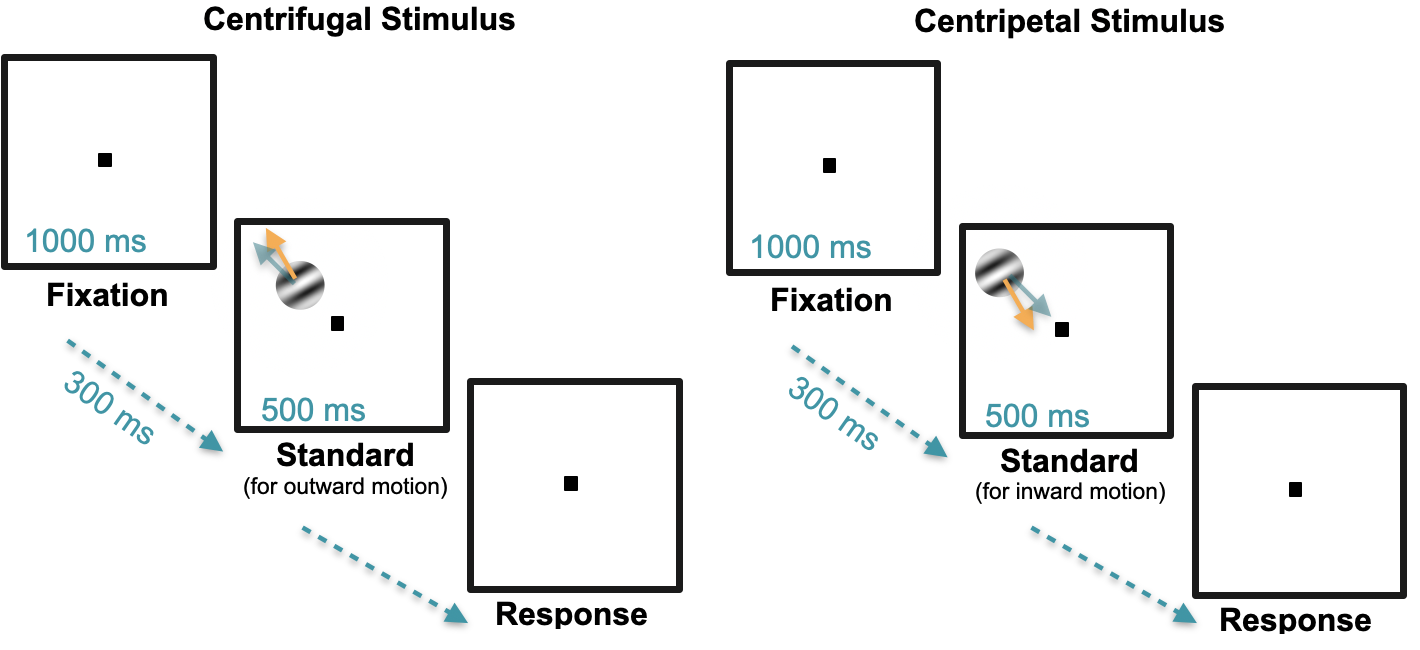
\includegraphics[scale=.4]{Images/Radial_sequence.png}
\\
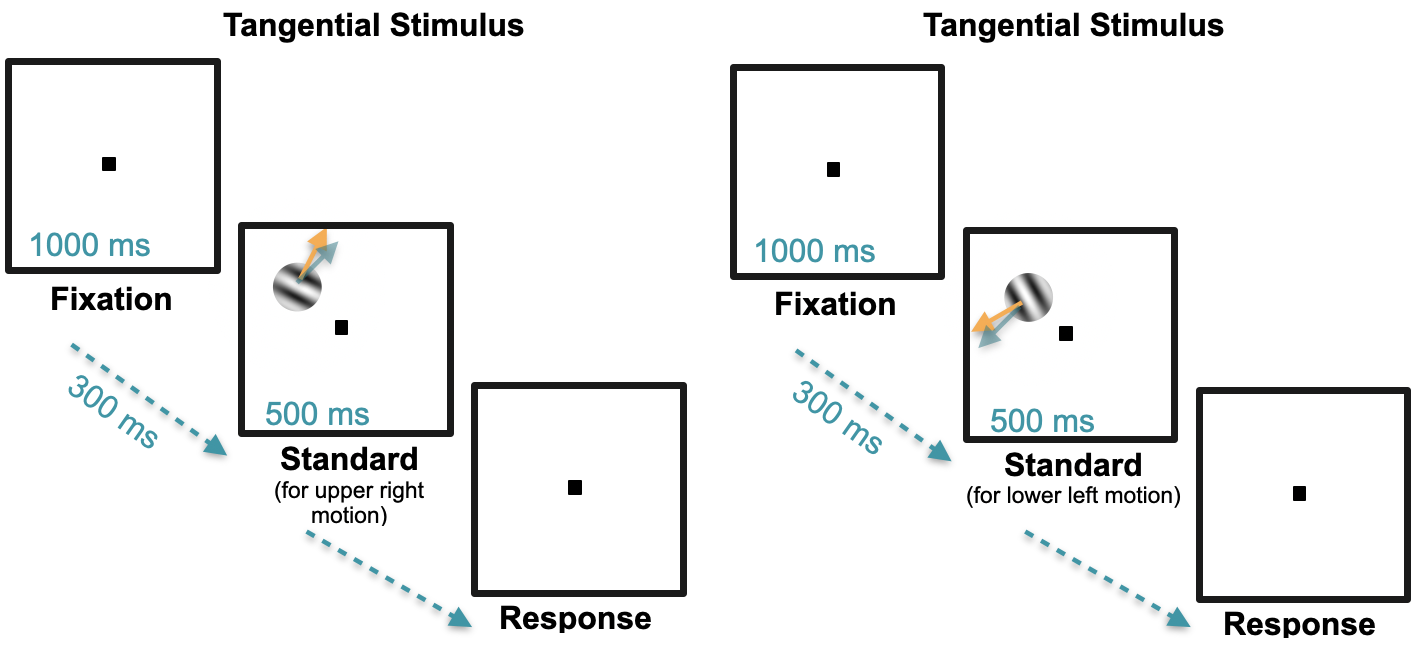
\includegraphics[scale=.4]{Images/Tang_sequence.png}
\caption{Blue arrow represents the internal reference, the orange arrow represents an example of the direction at which the stimulus is presented (can be clockwise or counterclockwise to the blue arrow.}
\end{figure}

\subsection{Block sequence}
Four blocks were run, and each block corresponded to 1 of the 4 conditions being tested (tangential lower left motion, tangential upper right motion, radial upper left motion, radial lower right motion). The internal reference frames for each block is shown below:

\begin{figure}[H]
\centering % centers the figure
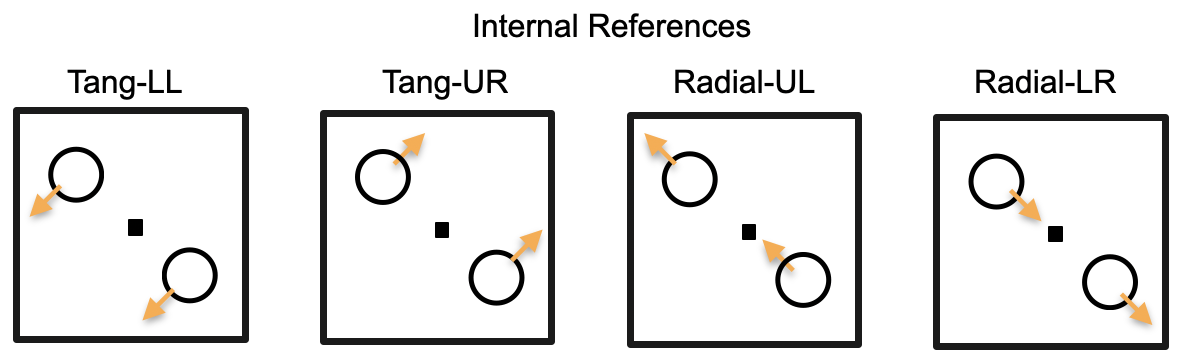
\includegraphics[scale=.4]{Images/Blocks.png}
\end{figure}

Prior to the experiment, the "standard" motion direction corresponding to that specific block is showed to the observer to use as an internal reference. Then a training session is conducted to determine how much tilt is required to meet 75\% accuracy with staircase procedure (MLPest), and to allow subject to practice task with feedback. This was tested using radial motion only, and ~1.5 degrees was the estimated angular value to add/subtract to the standard to achieve 75\% performance of the clockwise/counterclockwise discrimination task. Constants [-1.5, -1.25, -1, -0.75, -0.5, 0.5, 0.75, 1, 1.25, 1.5] were chosen to roughly center around this value for all 4 conditions. Note positive and negative values for clockwise v. counterclockwise tilt.
\\
%Each block contains (2 locations with clockwise/counterclockwise motion) x 80 repetitions = 1,280 trials. All 4 full-blocks took 80 min. 
Each condition (radial-in, radial-out, tang) contained 2 locations x 9 tilt values x 2 (clock v cc) x 20 repetitions = 720 trials. Each full-block takes ~35 min; all 3 full-blocks took 105 min. 
\\
RE Sequence of partial-blocks tested (re-test was in reverse order): 
\begin{enumerate}
\item radial-UL [angles: +- 0.5, 0.75, 1, 1.25, 1.5] (20 min, 40 trials) - BLOCK1a
\item radial-LR [angles: +- 0.5, 0.75, 1, 1.25, 1.5] (20 min, 40 trials) - BLOCK2a
\item tang-UR [angles: +- 0.5, 0.75, 1, 1.25, 1.5] (10 min, 20 trials) - BLOCK3a
\item tang-LL [angles: +- 0.5, 0.75, 1, 1.25, 1.5] (10 min, 20 trials) - BLOCK3b
\item tang-LL [angles: +- 2, 2.5, 3, 4] (8 min, 20 trials) - BLOCK3c
\item tang-UR [angles: +- 2, 2.5, 3, 4] (8 min, 20 trials) - BLOCK3d
\item radial-LR [angles: +- 2, 2.5, 3, 4] (15 min, 40 trials) - BLOCK2b
\item radial-UL [angles: +- 2, 2.5, 3, 4] (15 min, 40 trials) - BLOCK1b
\end{enumerate}
SK Sequence of partial-blocks tested (re-test was in reverse order): 
\begin{enumerate}
\item radial-UL [angles: +- 0.5, 1, 1.5, 2.5, 4] (20 min, 40 trials) - BLOCK1
\item radial-LR [angles: +- 0.5, 1, 1.5, 2.5, 4] (20 min, 40 trials) - BLOCK2
\item tang-UR [angles: +- 0.5, 1, 1.5, 2.5, 4] (10 min, 20 trials) - BLOCK3
\item tang-LL [angles: +- 0.5, 1, 1.5, 2.5, 4] (10 min, 20 trials) - BLOCK3
\end{enumerate}

\newpage
\section{Data}
\subsection{Psychometric Function (Cumulative normal)}
\begin{figure}[H]
\centering % centers the figure
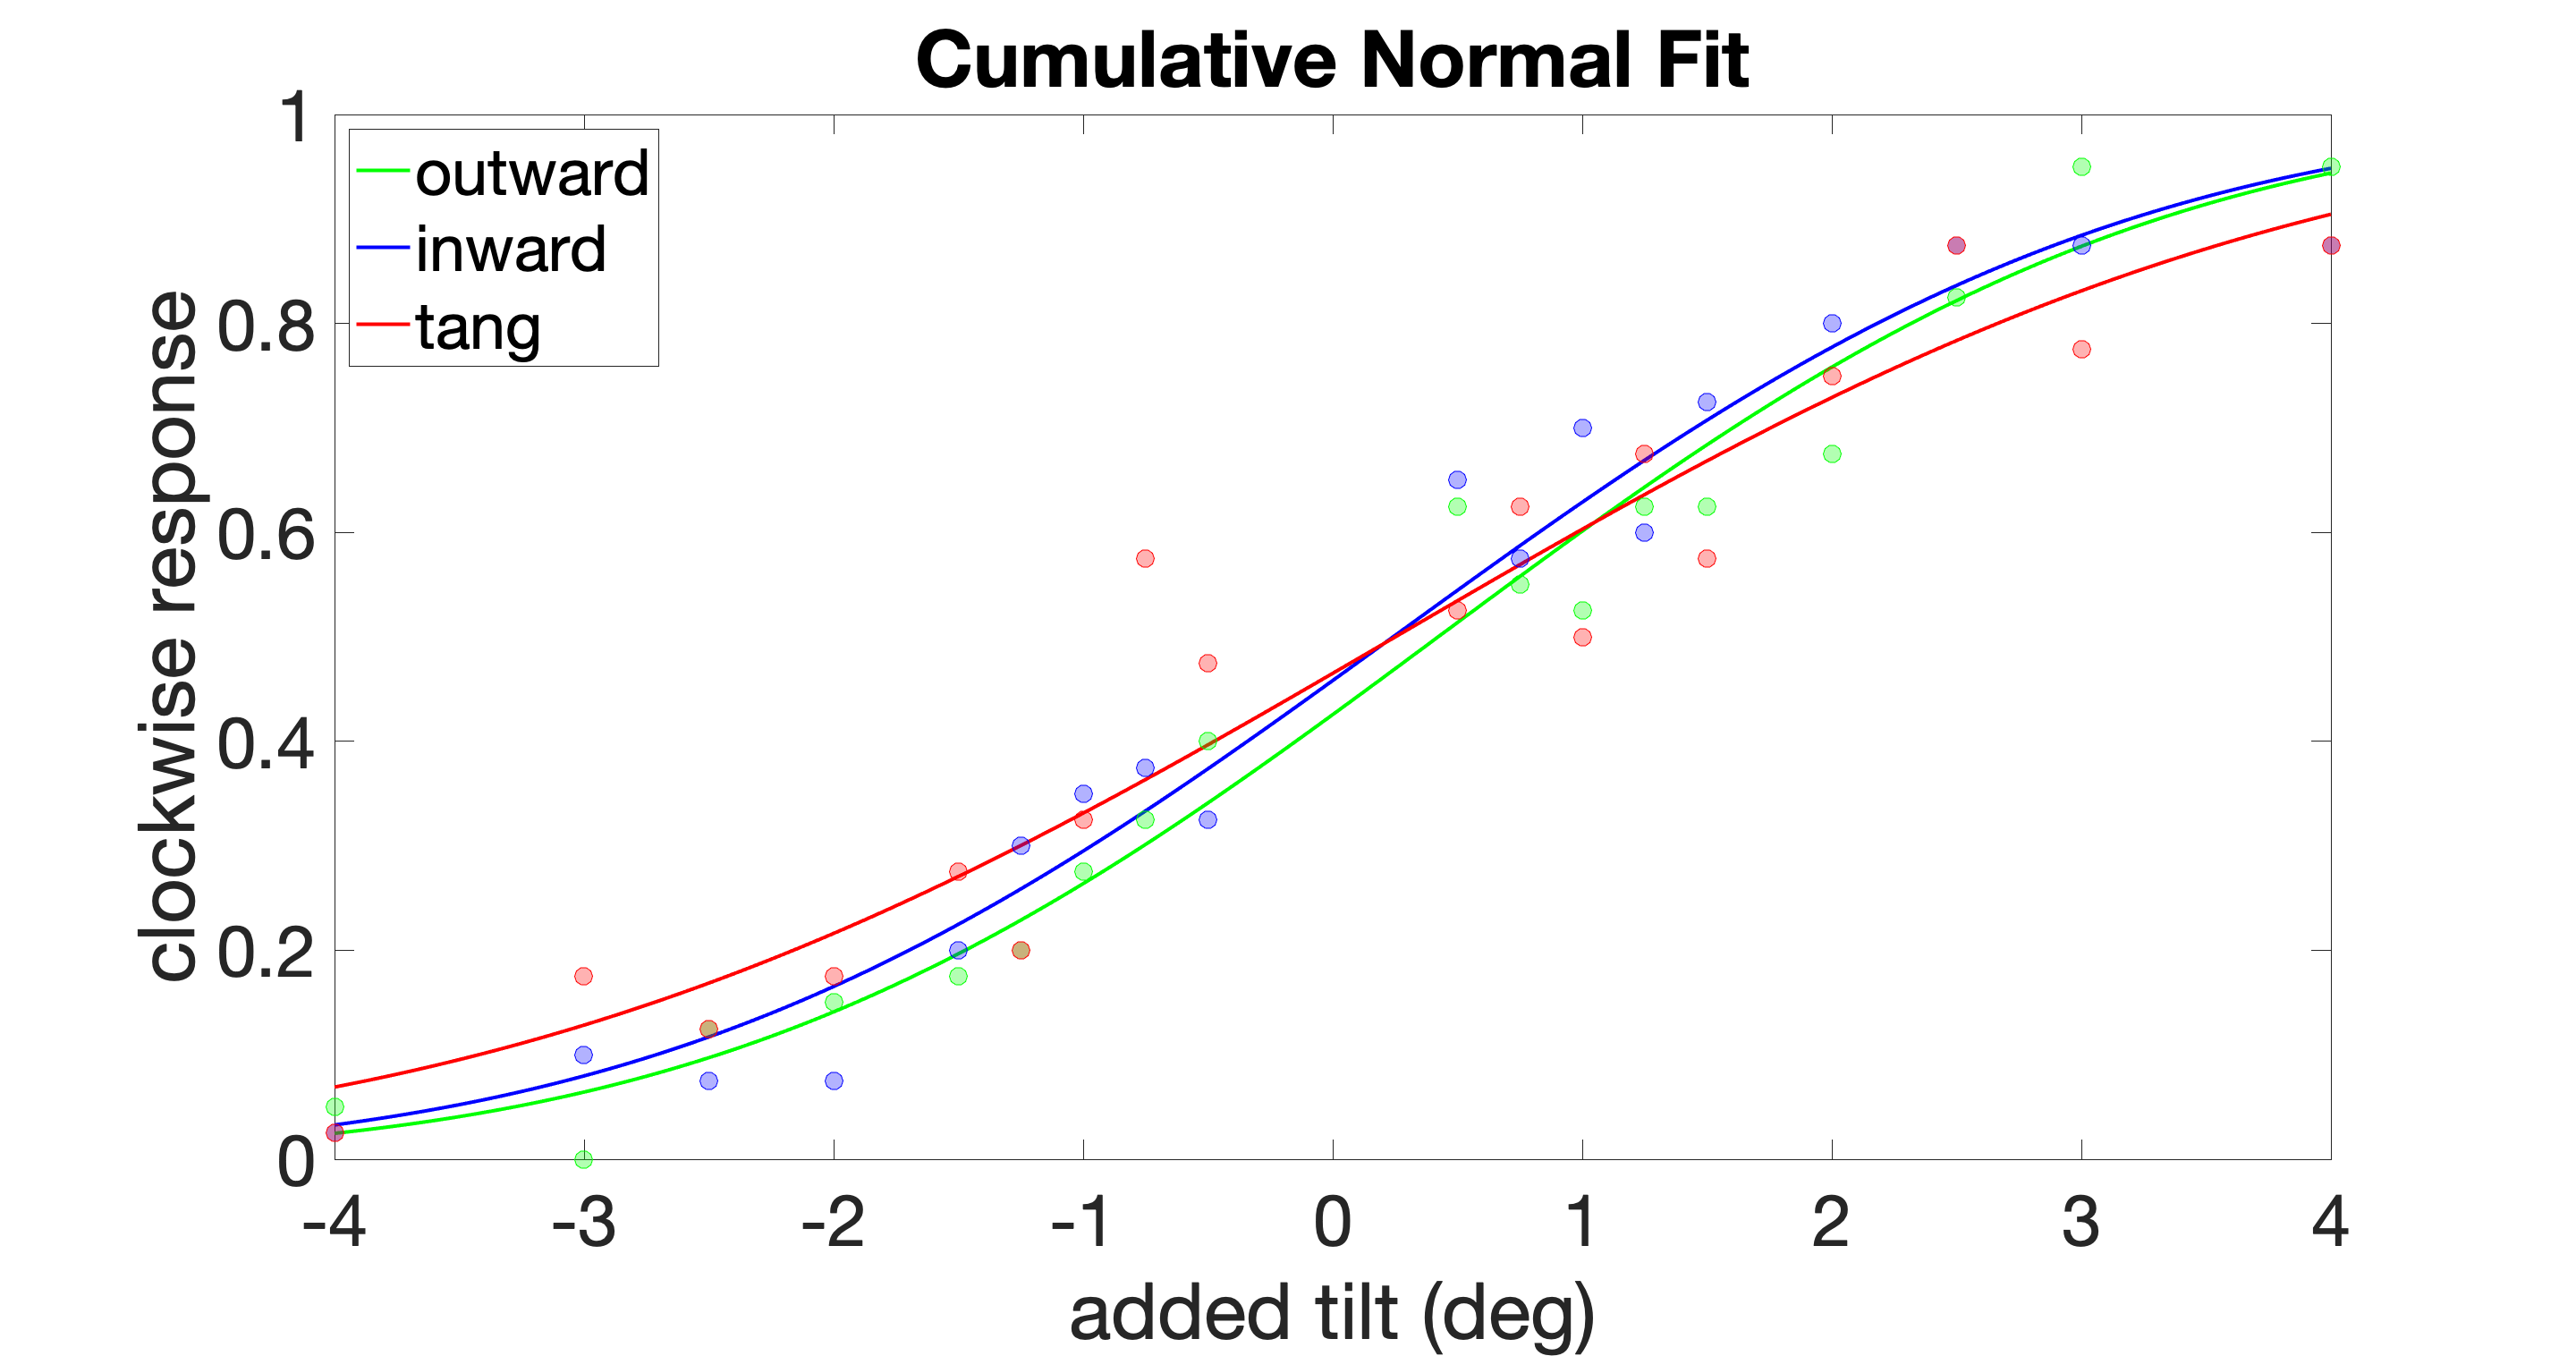
\includegraphics[scale=.08]{Images/PF_set1.png}
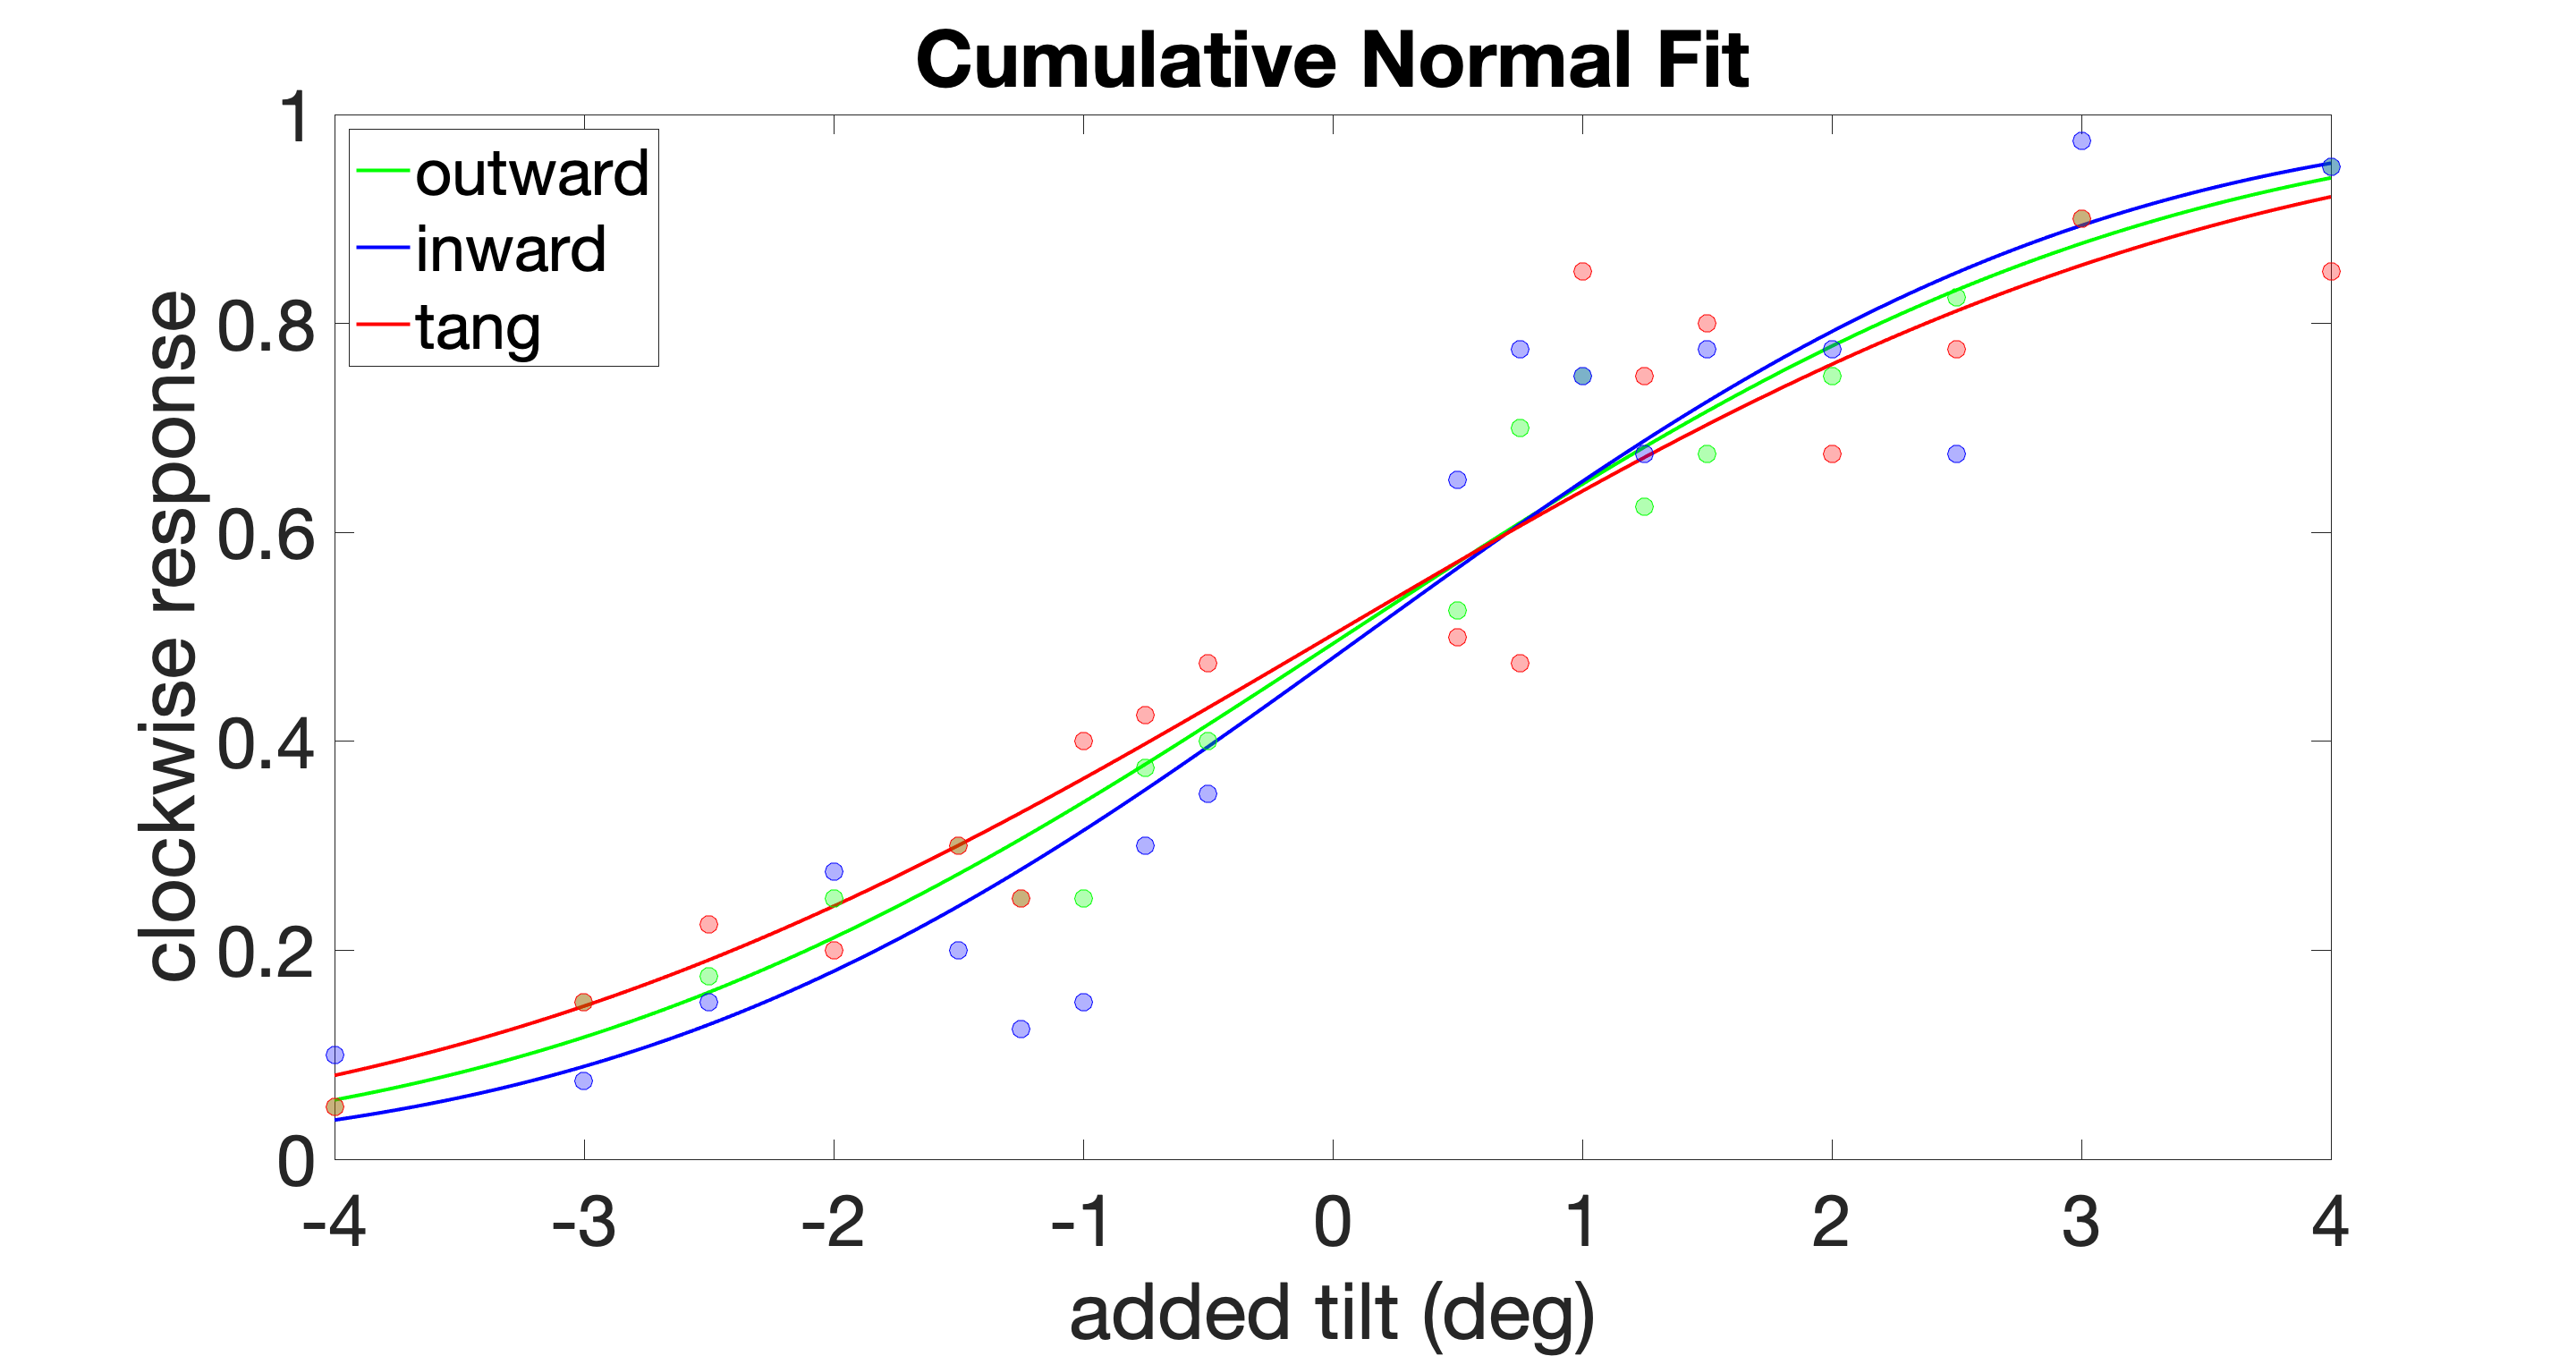
\includegraphics[scale=.08]{Images/PF_set2.png}
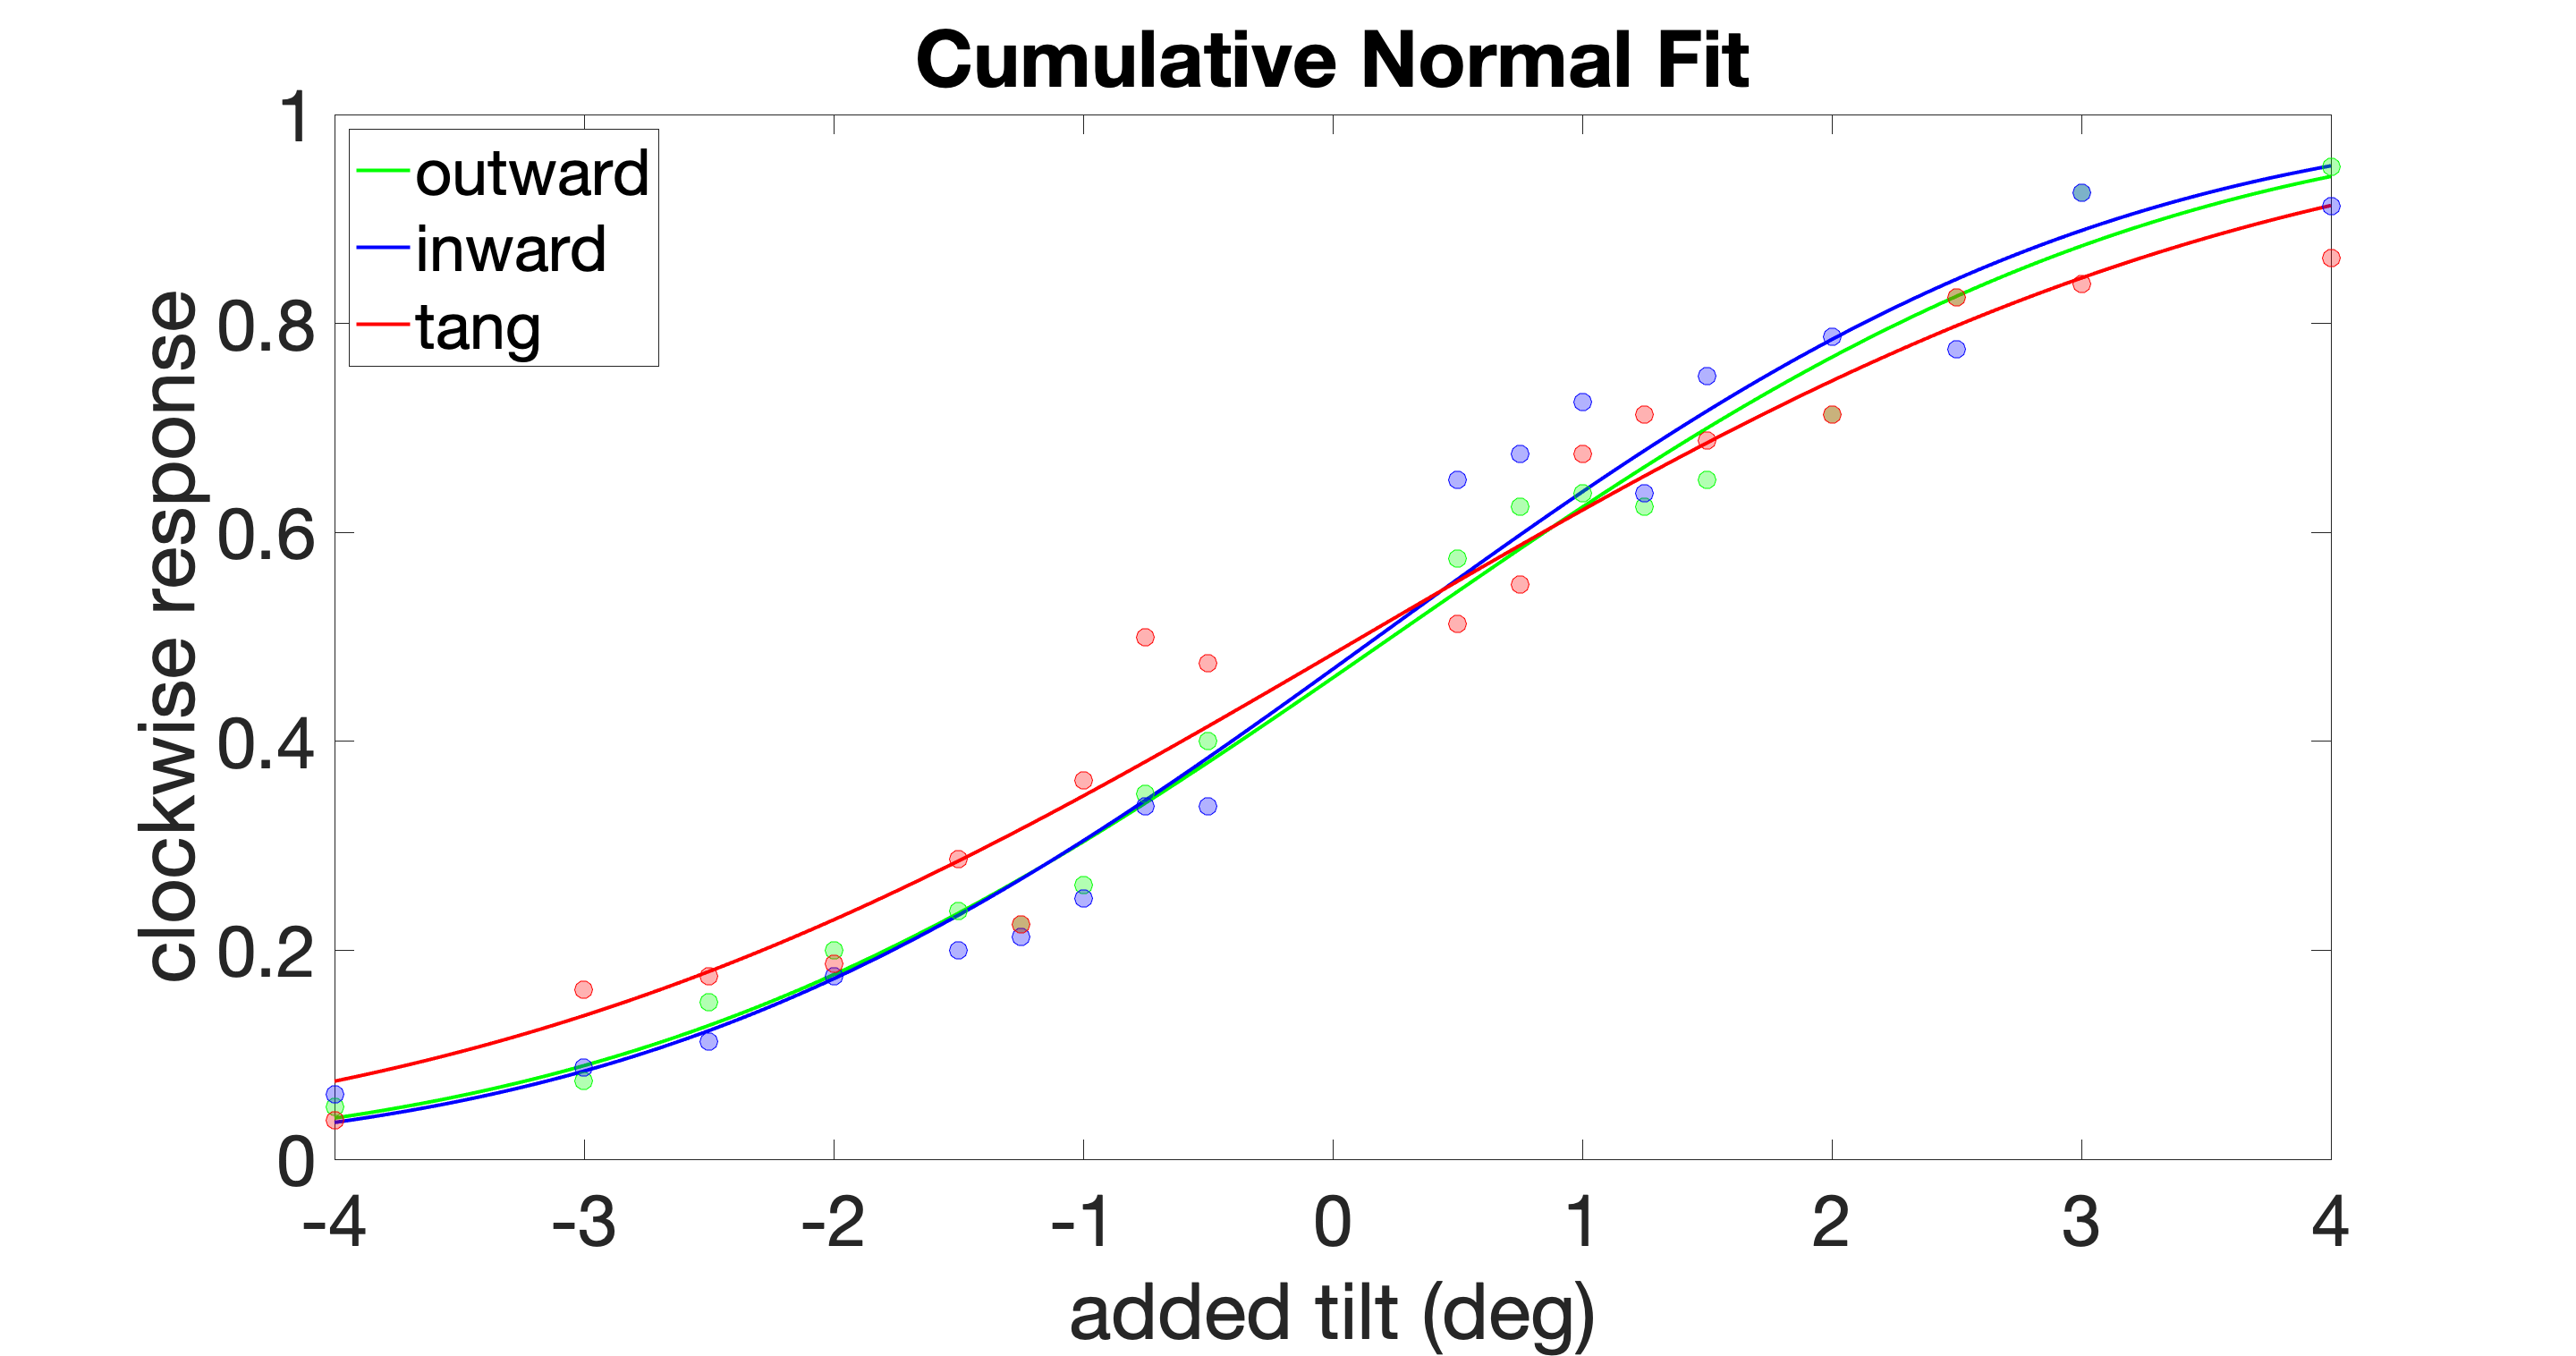
\includegraphics[scale=.08]{Images/PF_combined.png}
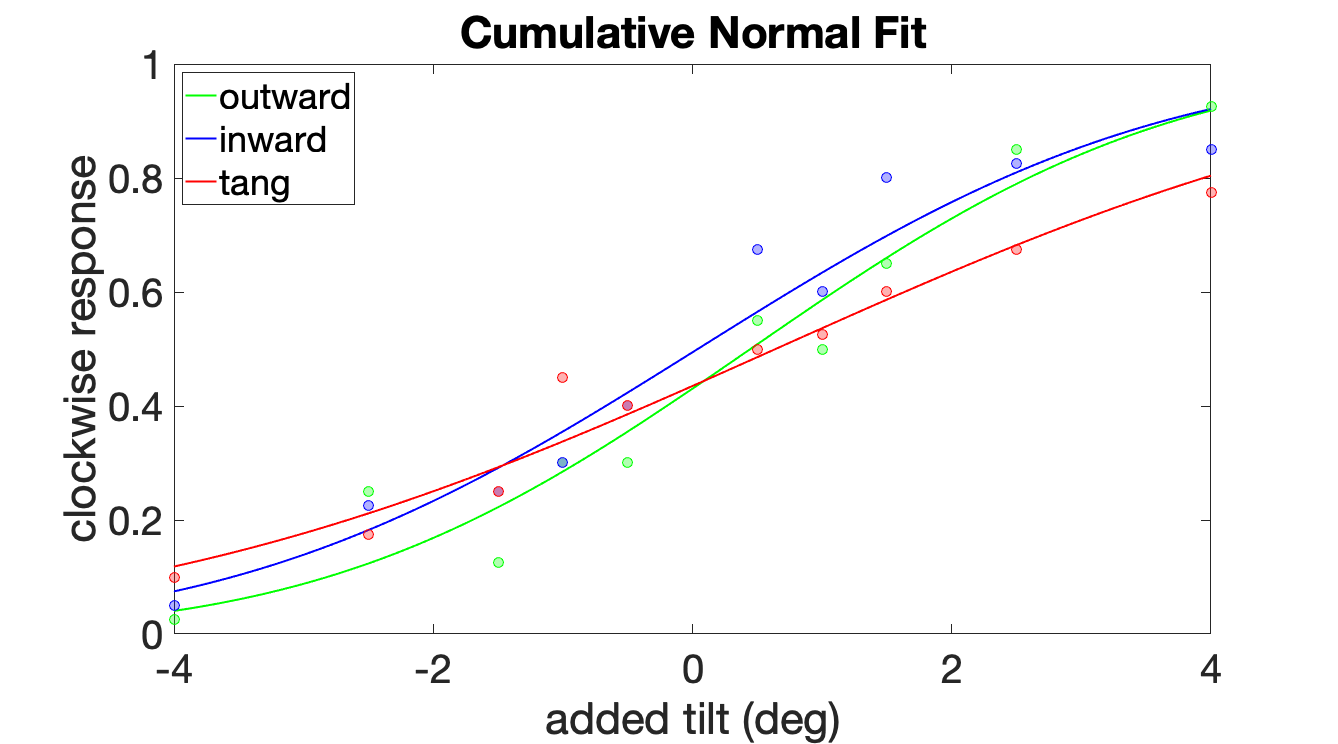
\includegraphics[scale=.16]{Images/PF_SK.png}
\caption{Top left: RE test data with blocks that contain same reference vector; combines data across locations (40 trials per angle). Top right: RE re-test with same number of trials. Bottom left: combined RE test \& re-test data from top row (80 trials per angle). Bottom right: SK data tested with evenly distributed difficulty levels of 1 internal reference per block (40 trials).}
\end{figure}

\textbf{RE SENSITIVIY/SLOPE}
\\
Radial out beta = [test 0.4441], [re-test 0.3914], [combined 0.4149]
\\
Radial in beta = [test 0.4339], [re-test 0.4324], [combined 0.4328]
\\
Tangential beta = [test 0.3488], [re-test 0.3521], [combined 0.3501]
\\
\textbf{RE BIAS}
\\
Radial out alpha = [test 0.4225]; [re-test 0.0425], [combined 0.2376]
\\
Radial in alpha = [test 0.242]; [re-test 0.1172], [combined 0.1787]
\\
Tangential alpha = [test 0.2512]; [re-test -0.014], [combined 0.1183]
\\
\textbf{SK SENSITIVIY/SLOPE}
\\
Radial out beta = [test 0.3924]
\\
Radial in beta = [test 0.3567]
\\
Tangential beta = [test 0.2550]
\\
\textbf{SK BIAS}
\\
Radial out alpha = [test 0.4467]
\\
Radial in alpha = [test 0.0404]
\\
Tangential alpha = [test 0.6407]

\newpage
\subsection{Mean Slope \& CI}
\begin{figure}[H]
\centering % centers the figure
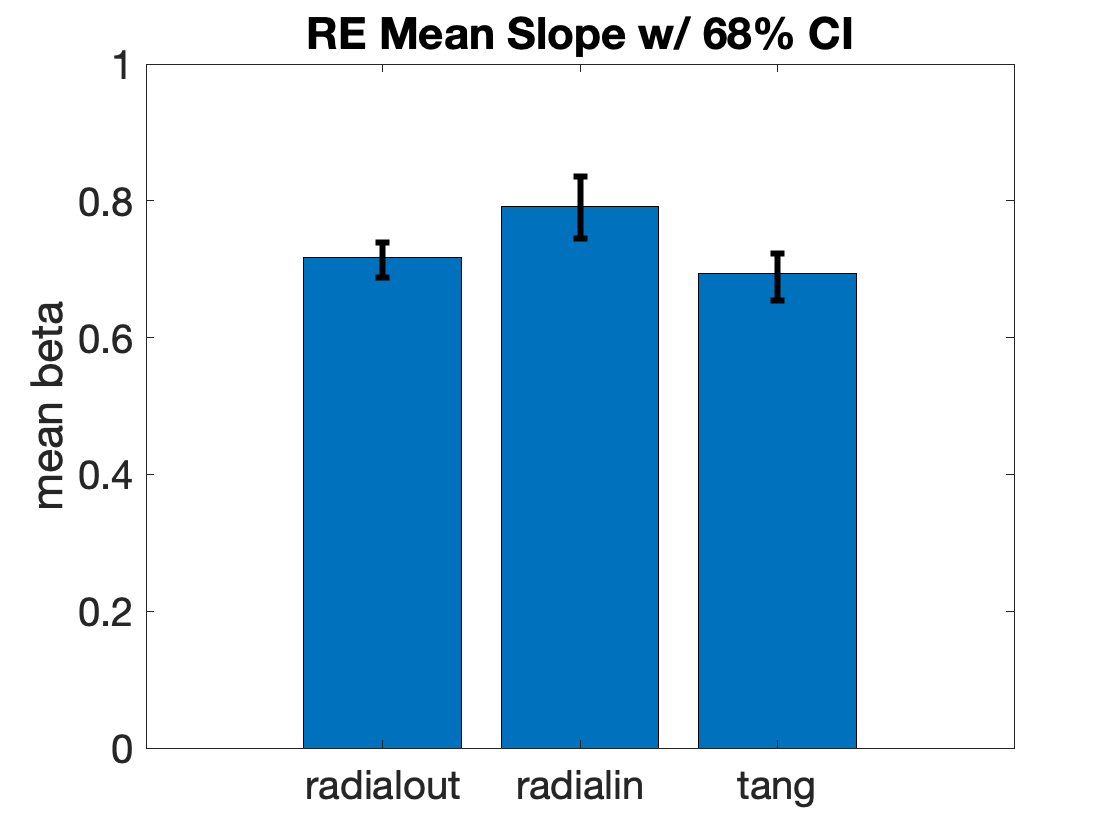
\includegraphics[scale=.2]{Images/MeanSlopeError_68ci_RE.png}
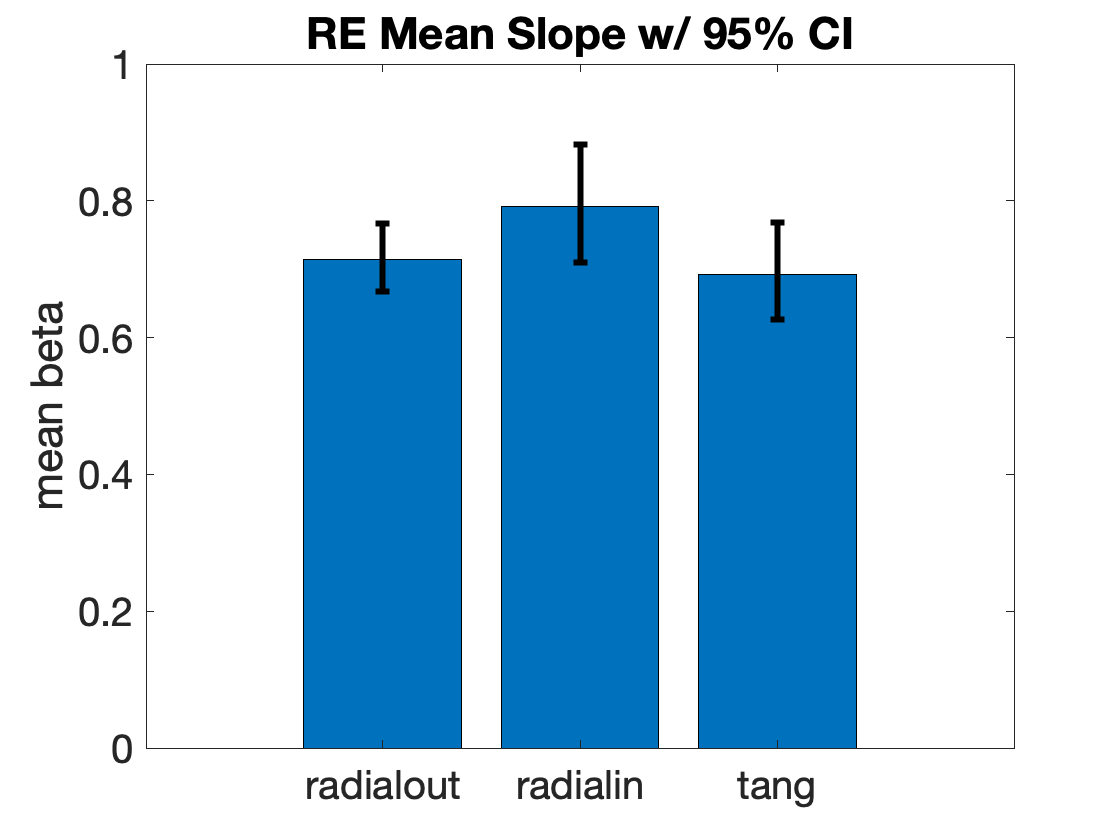
\includegraphics[scale=.2]{Images/MeanSlopeError_95ci_RE.png}
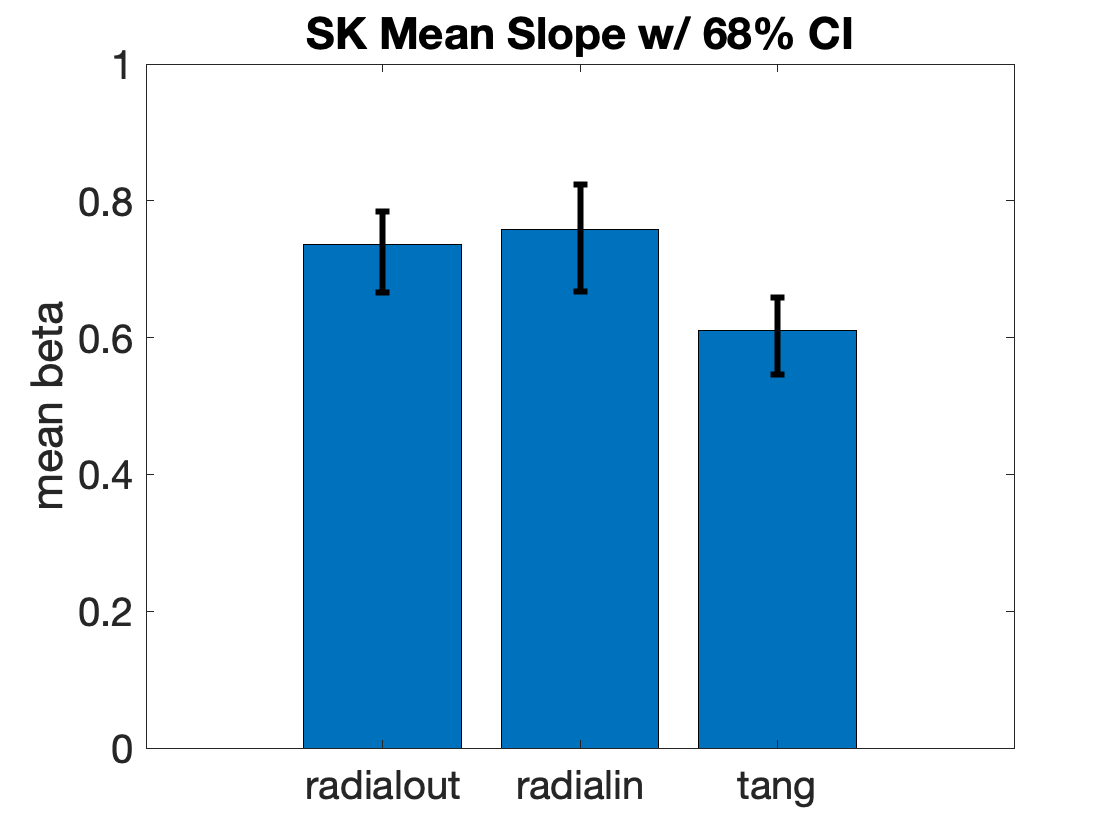
\includegraphics[scale=.2]{Images/MeanSlopeError_68ci_SK.png}
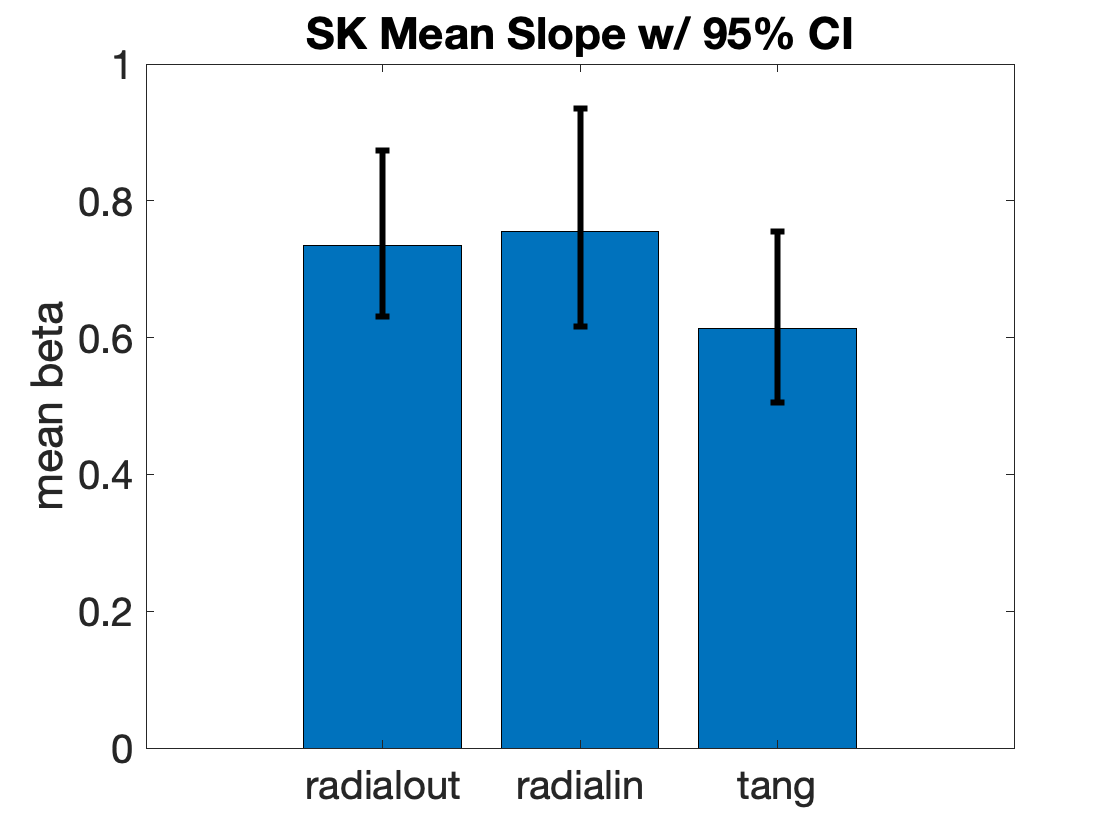
\includegraphics[scale=.2]{Images/MeanSlopeError_95ci_SK.png}
\caption{Top right/left: RE data (80 trails per angle). Lower right/left: SK data (40 trials per angle). These means/confidence intervals were computed from samples of posterior distribution using Markov chain Monte Carlo method (from PAL\_PFHB\_fitModel.m) - 5000 samples, 3 chains.}
\end{figure}

\subsection{Mean Bias \& CI}
\begin{figure}[H]
\centering % centers the figure
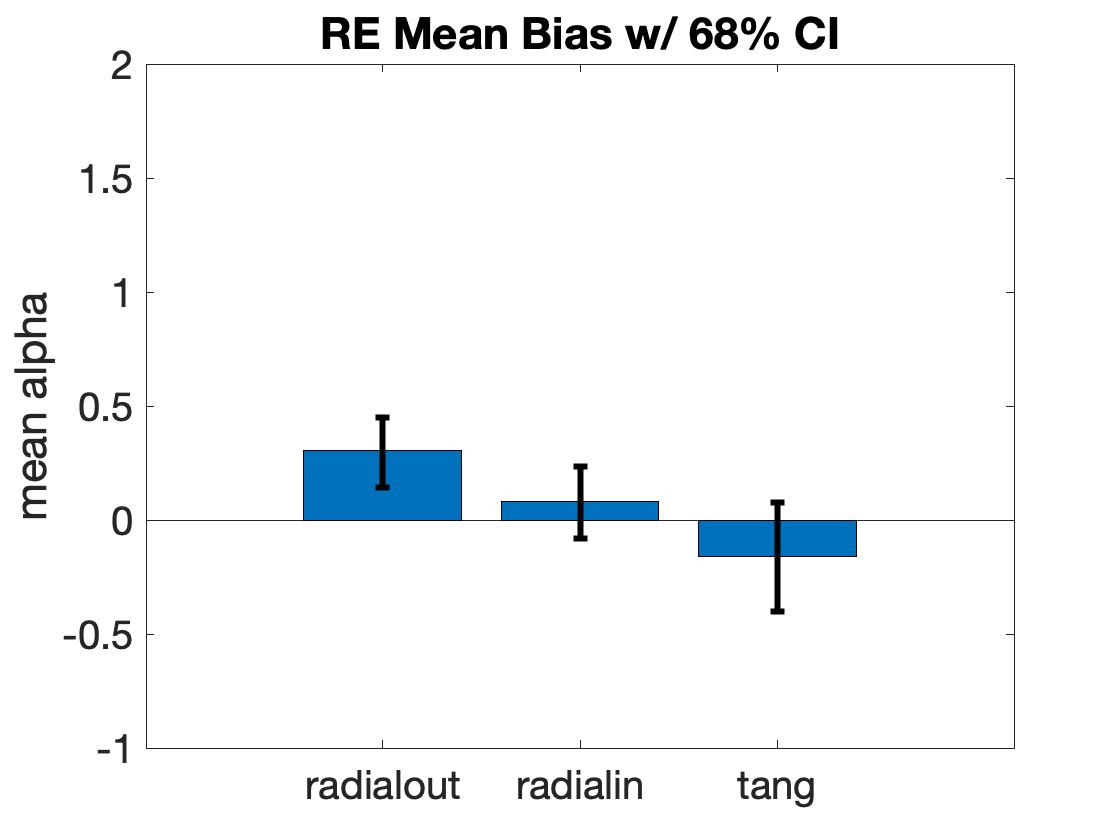
\includegraphics[scale=.2]{Images/MeanBiasError_68ci_RE.png}
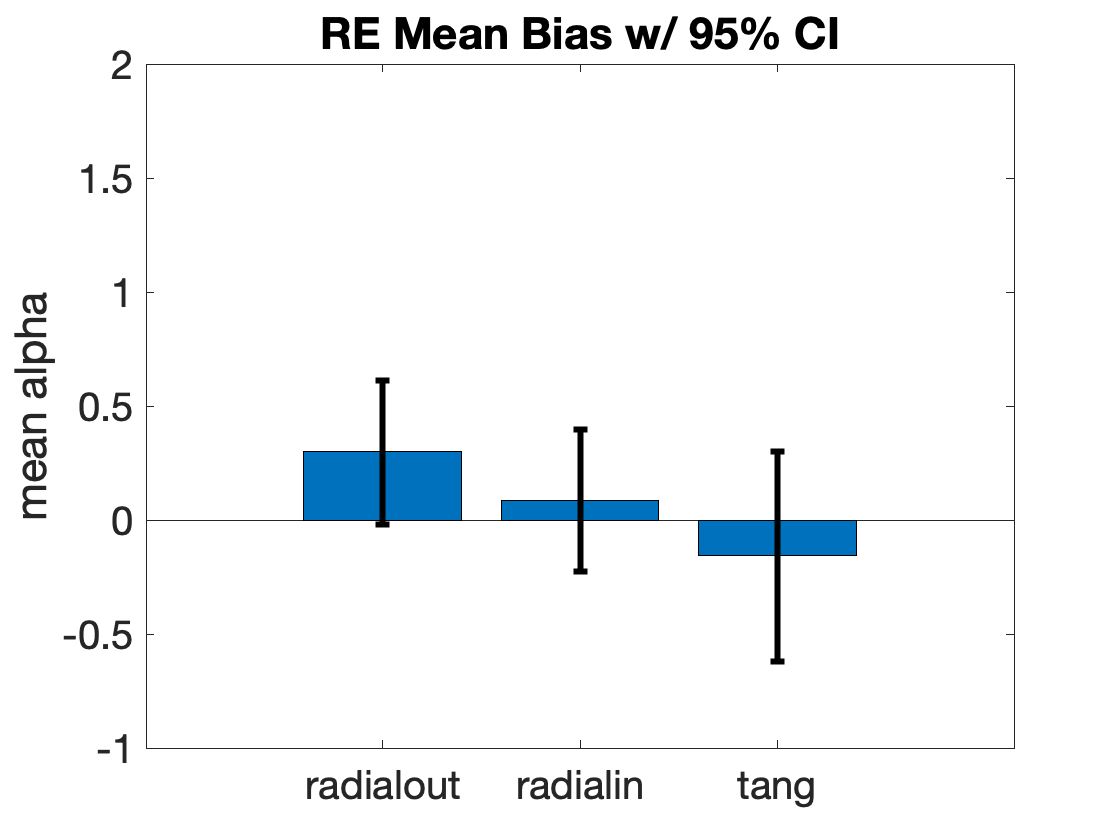
\includegraphics[scale=.2]{Images/MeanBiasError_95ci_RE.png}
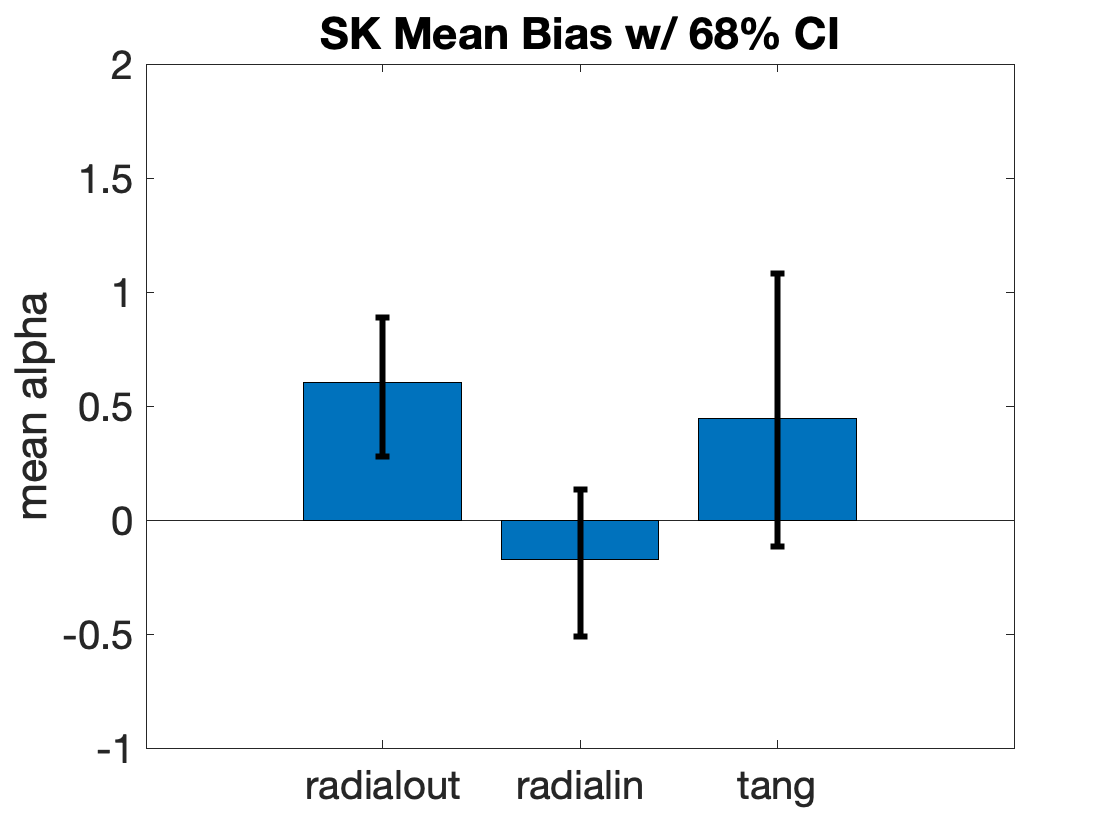
\includegraphics[scale=.2]{Images/MeanBiasError_68ci_SK.png}
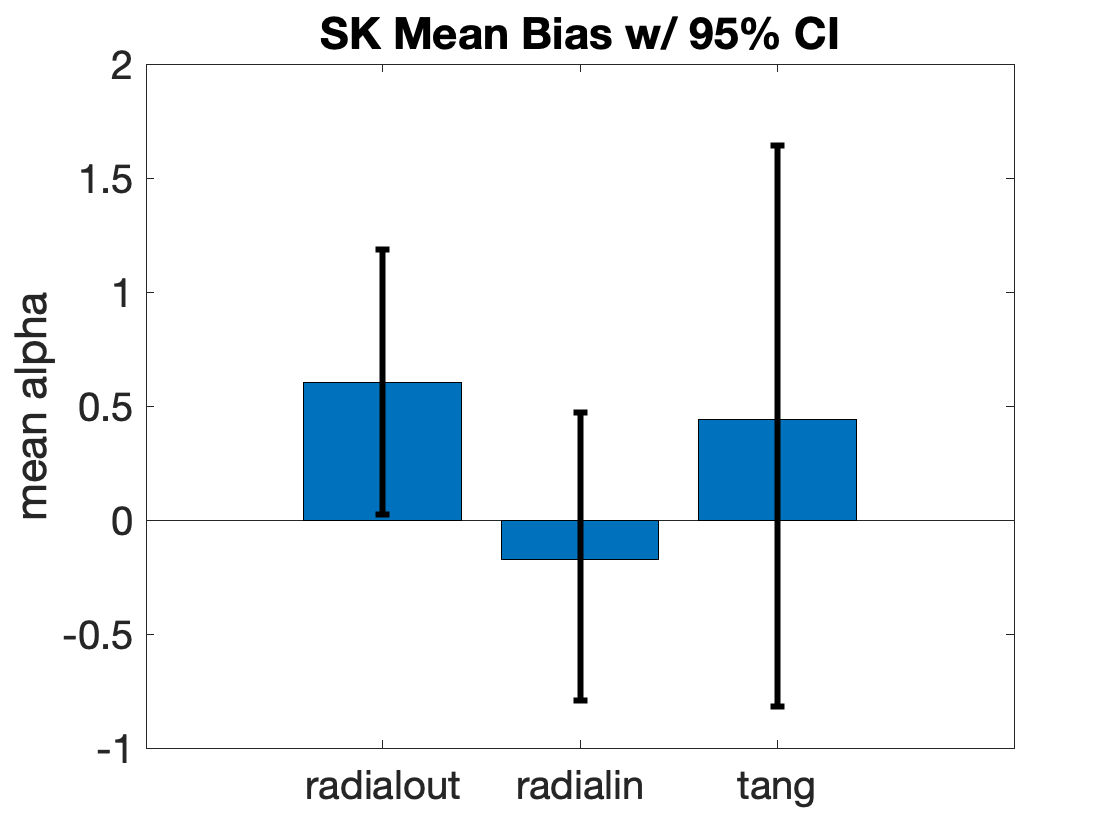
\includegraphics[scale=.2]{Images/MeanBiasError_95ci_SK.png}
\caption{Top right/left: RE data (80 trails per angle). Lower right/left: SK data (40 trials per angle). These means/confidence intervals were computed from samples of posterior distribution using Markov chain Monte Carlo method (from PAL\_PFHB\_fitModel.m) - 5000 samples, 3 chains.}
\end{figure}

\newpage
\subsection{TESTING SPEED 6.5 deg / s (eccentricity = 7 deg)}
\begin{figure}[H]
\centering % centers the figure
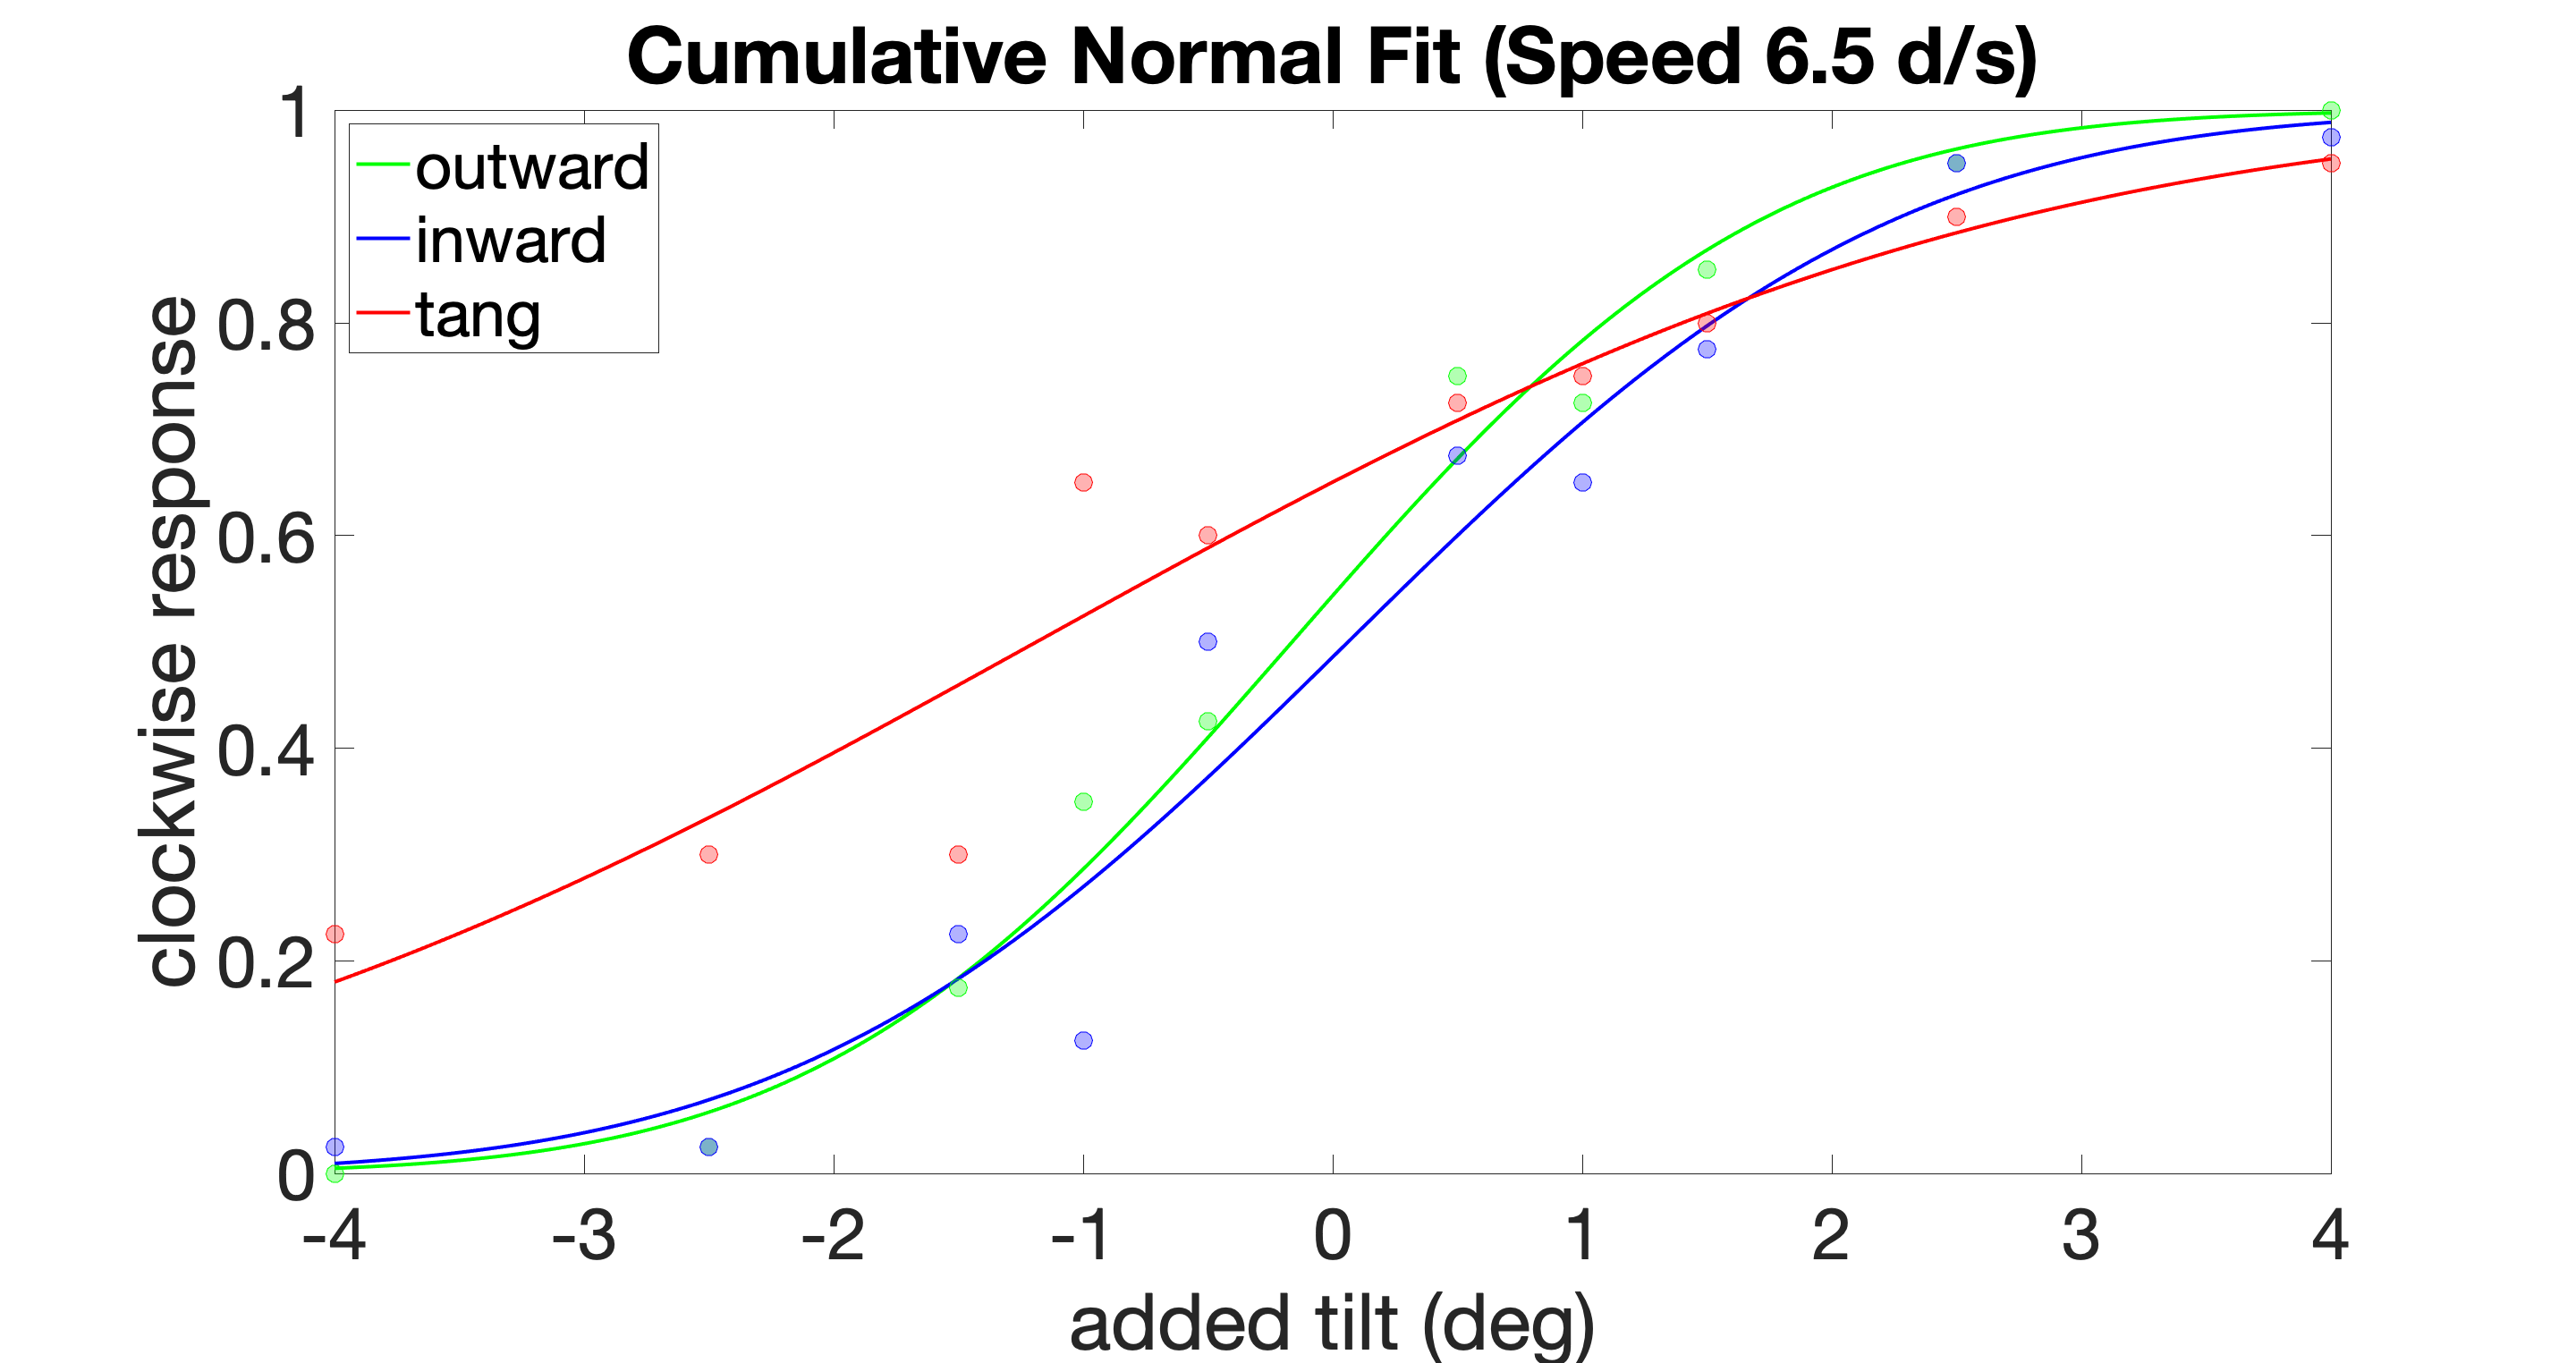
\includegraphics[scale=.08]{Images/PF_speed6.5.png}
\\
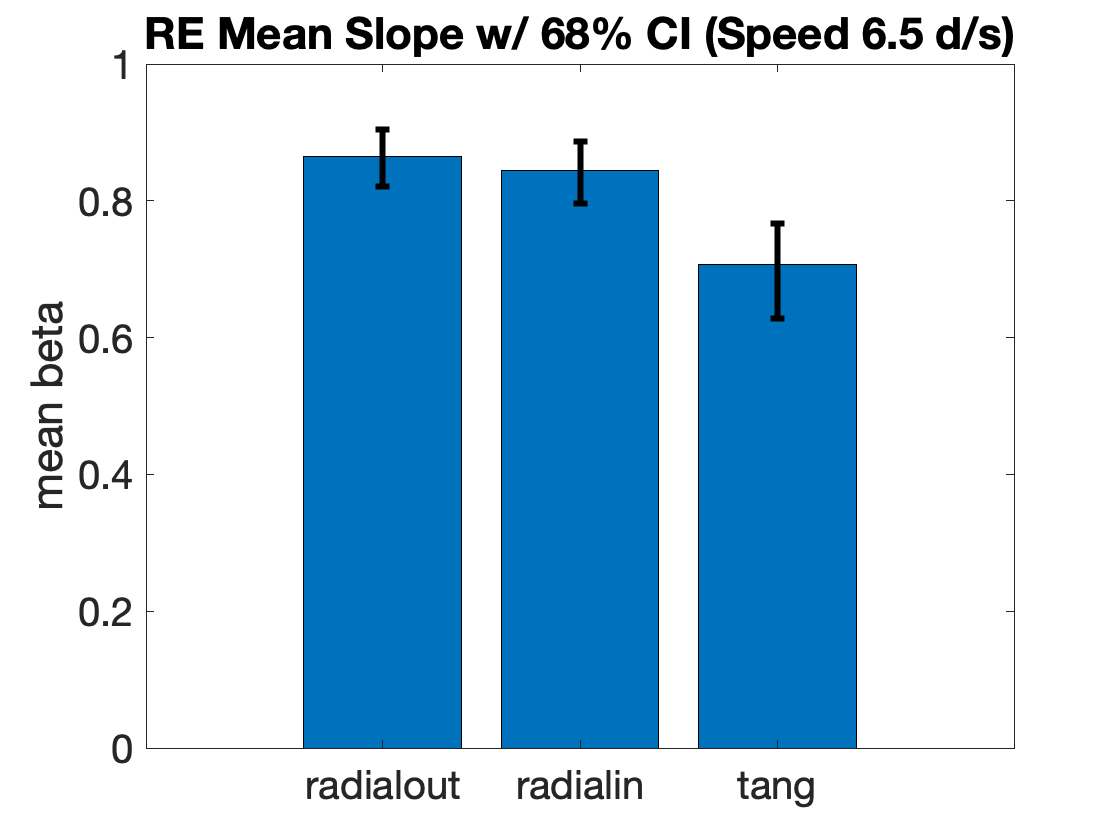
\includegraphics[scale=.2]{Images/MeanSlopeError_68ci_RE_speed6.5.png}
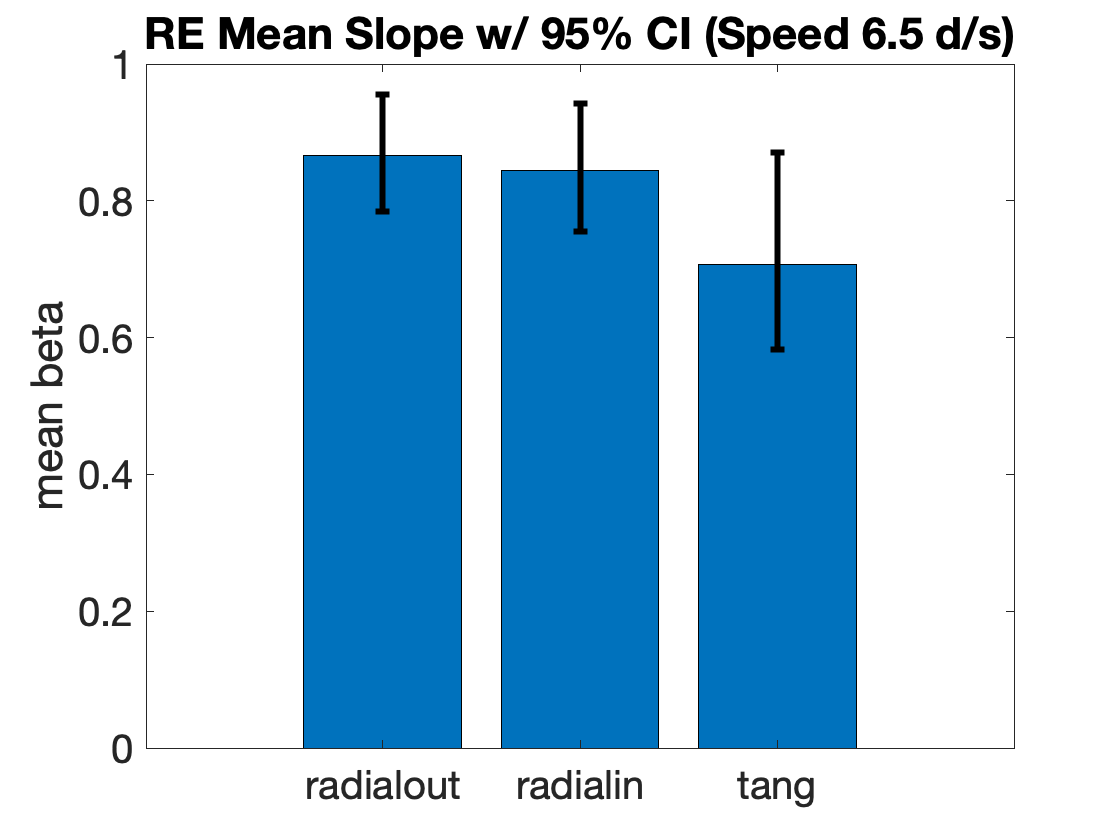
\includegraphics[scale=.2]{Images/MeanSlopeError_95ci_RE_speed6.5.png}
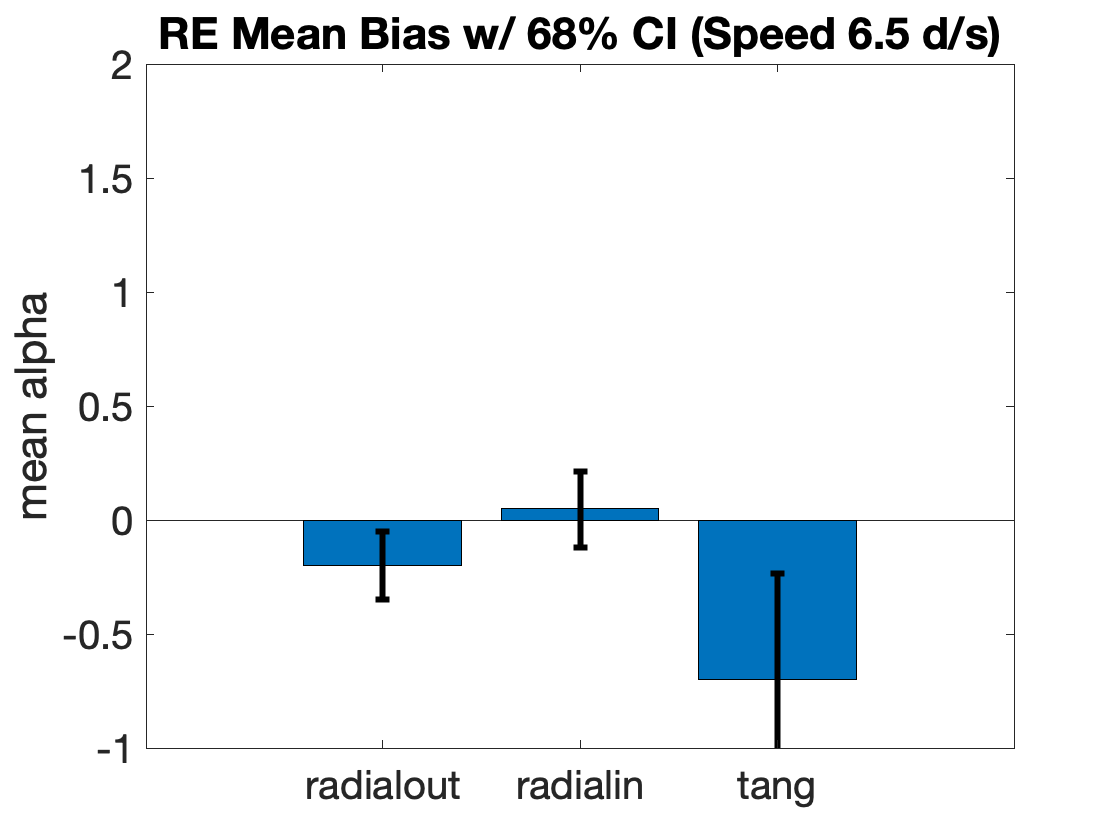
\includegraphics[scale=.2]{Images/MeanBiasError_68ci_RE_speed6.5.png}
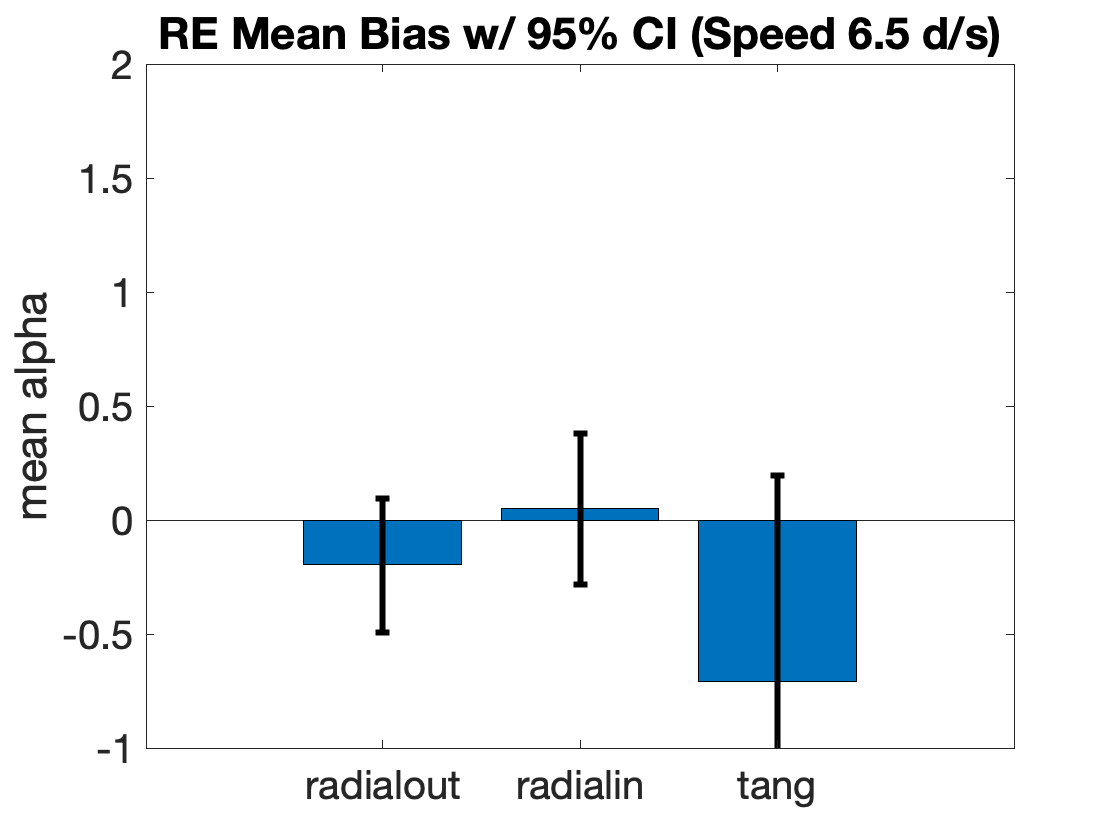
\includegraphics[scale=.2]{Images/MeanBiasError_95ci_RE_speed6.5.png}
\caption{Top right/left: RE data (40 trails per angle -- new data).  Same layout as previous pages, but for speed 6.5 deg /s. Note: not all angles tested.}
\end{figure}

\newpage
\subsection{TESTING ECCENTRICITY 14 deg (speed = 4 deg / s)}
\begin{figure}[H]
\centering % centers the figure
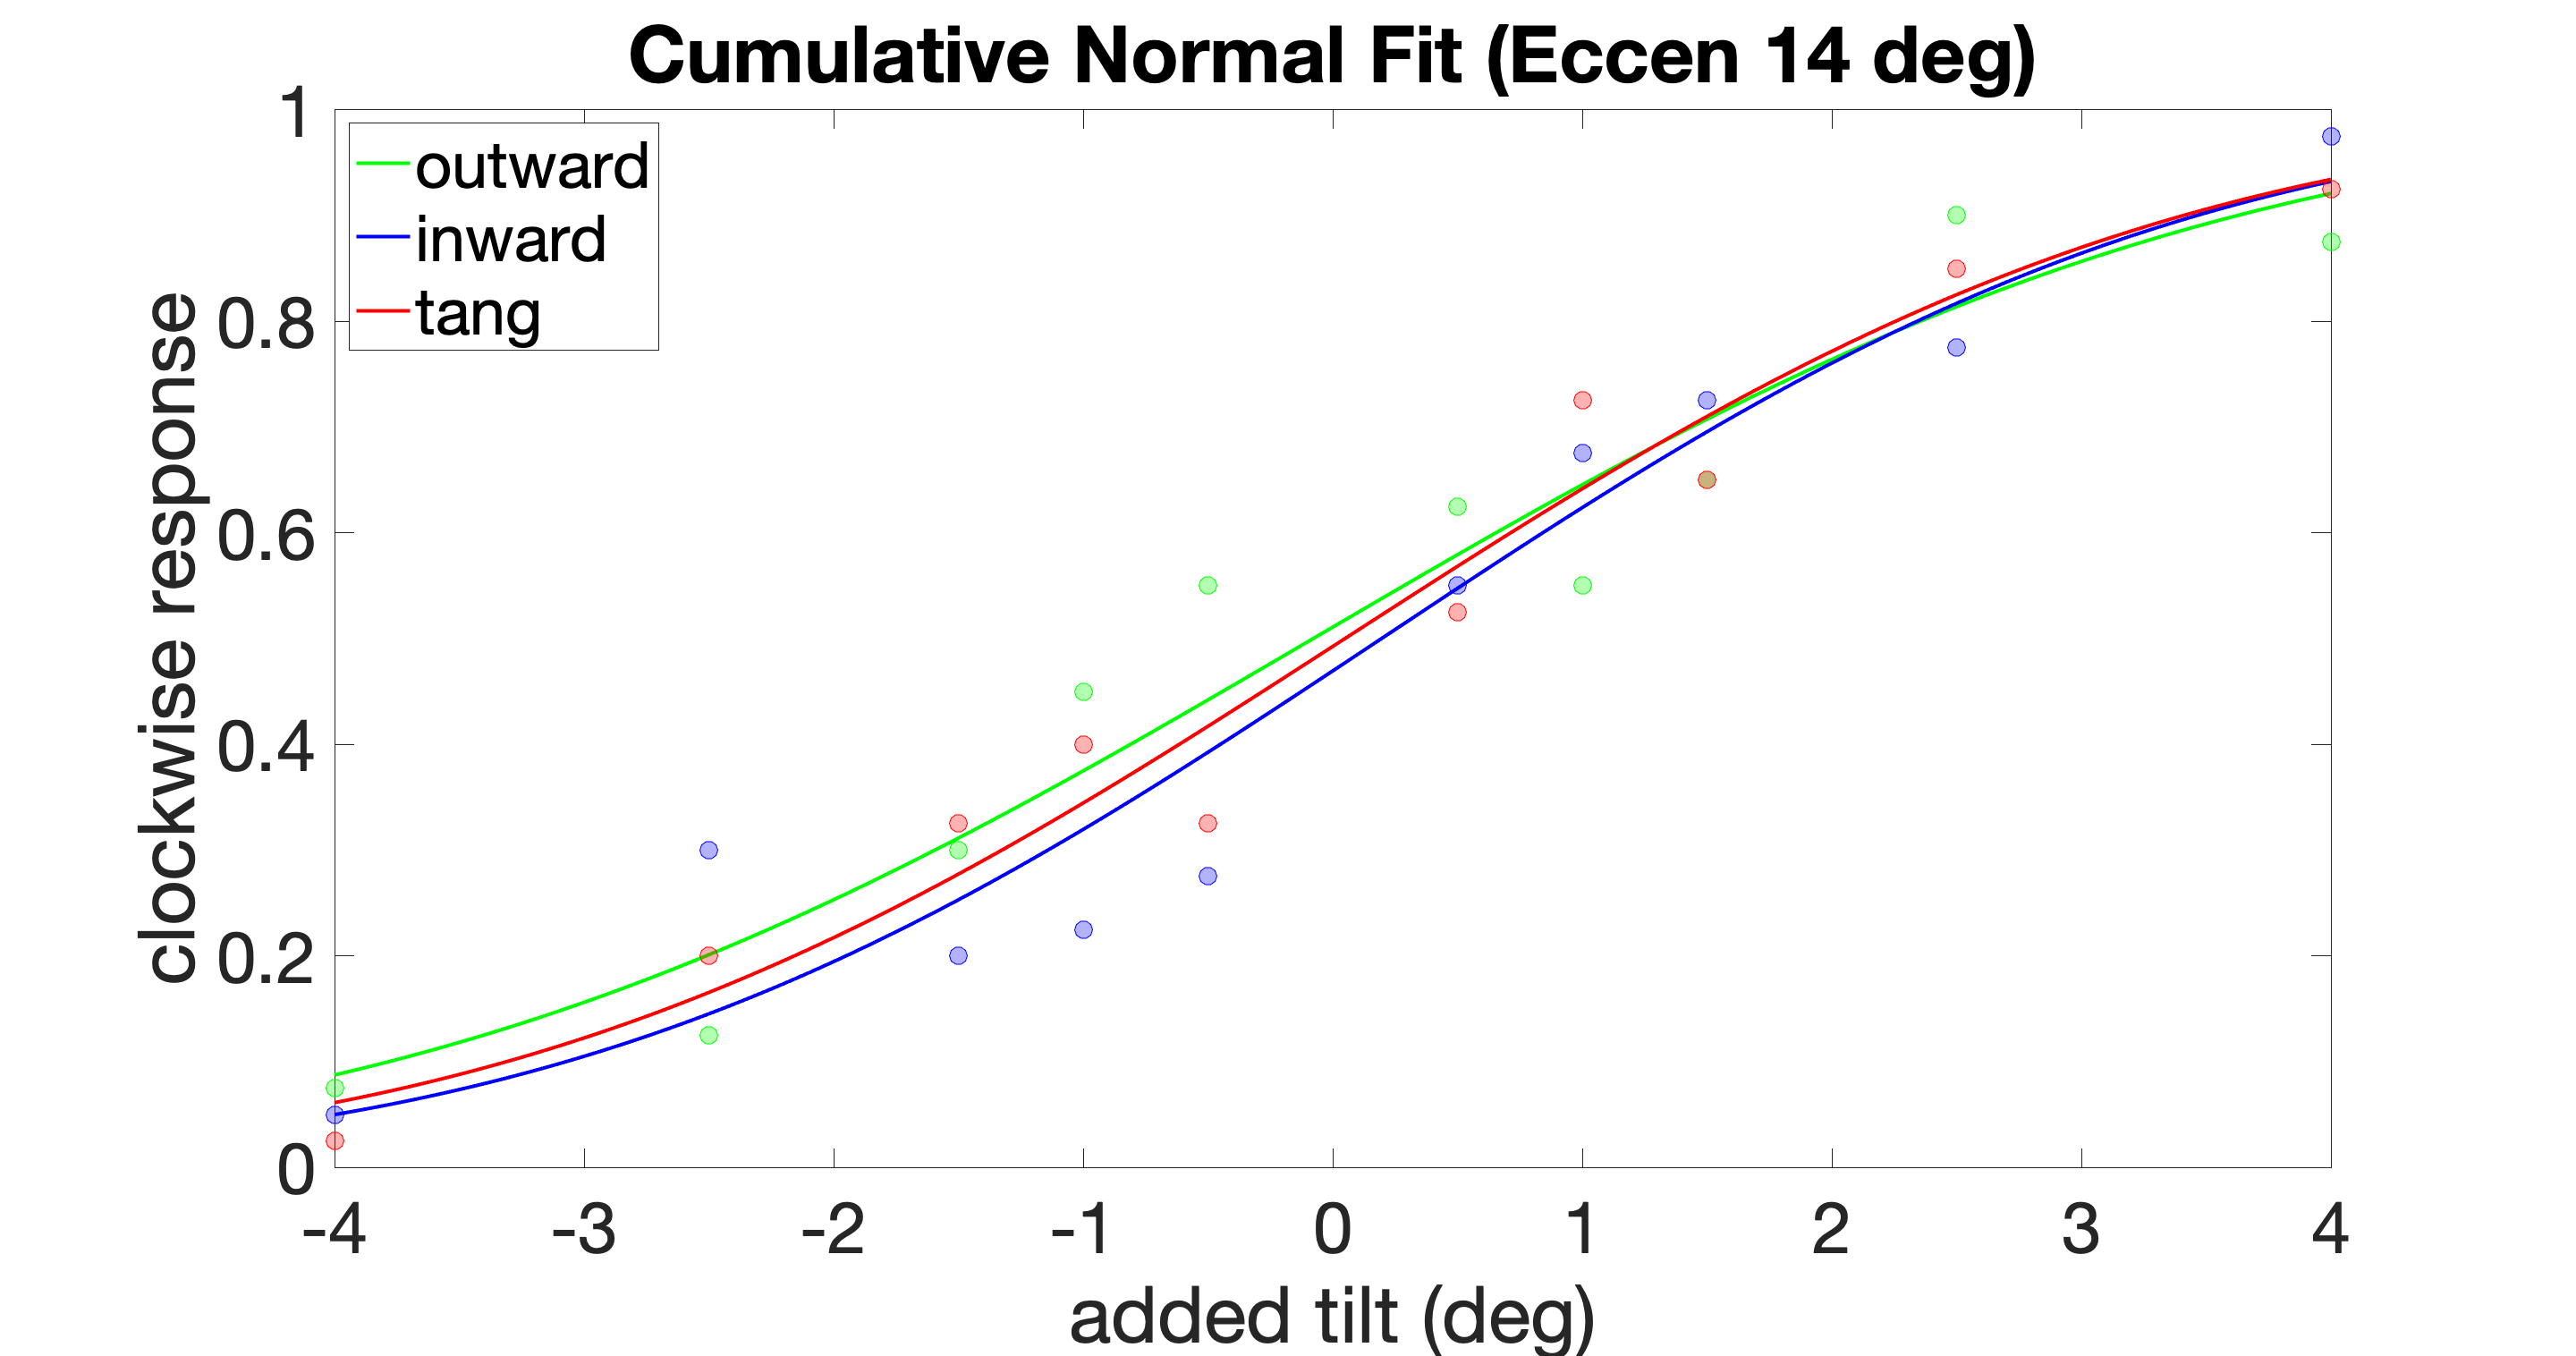
\includegraphics[scale=.08]{Images/PF_eccen14.png}
\\
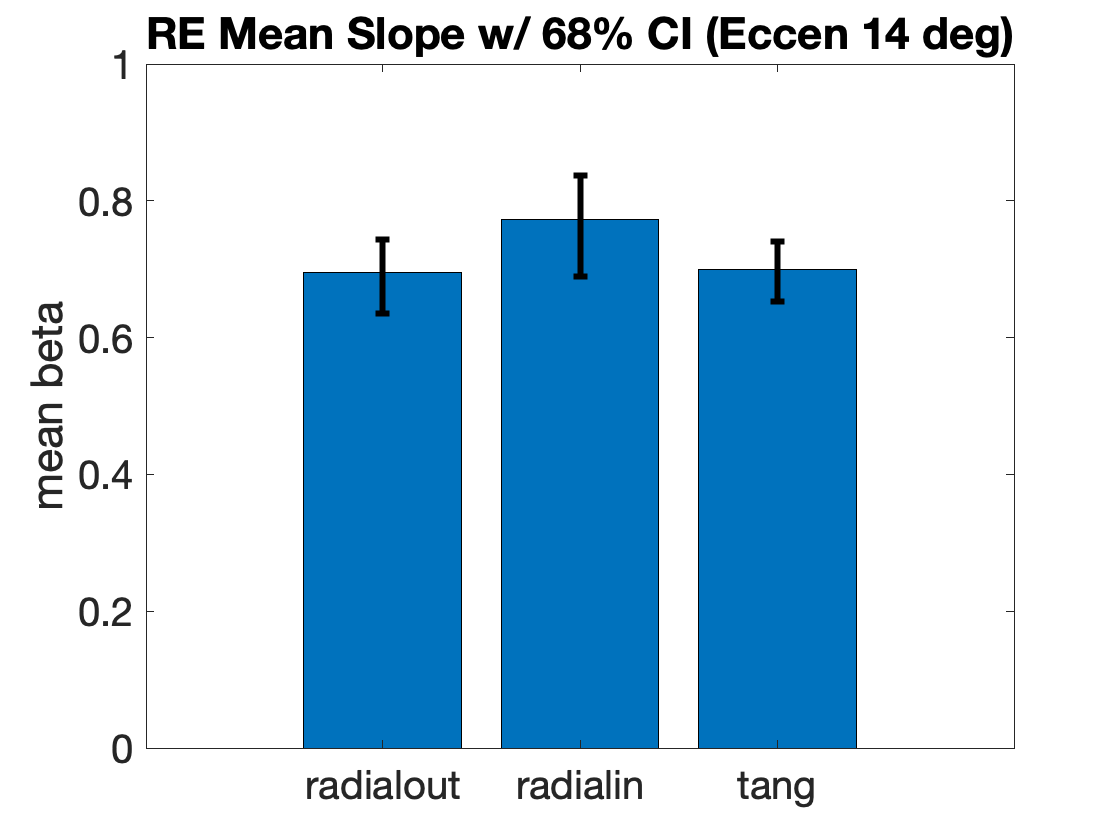
\includegraphics[scale=.2]{Images/MeanSlopeError_68ci_RE_eccen14.png}
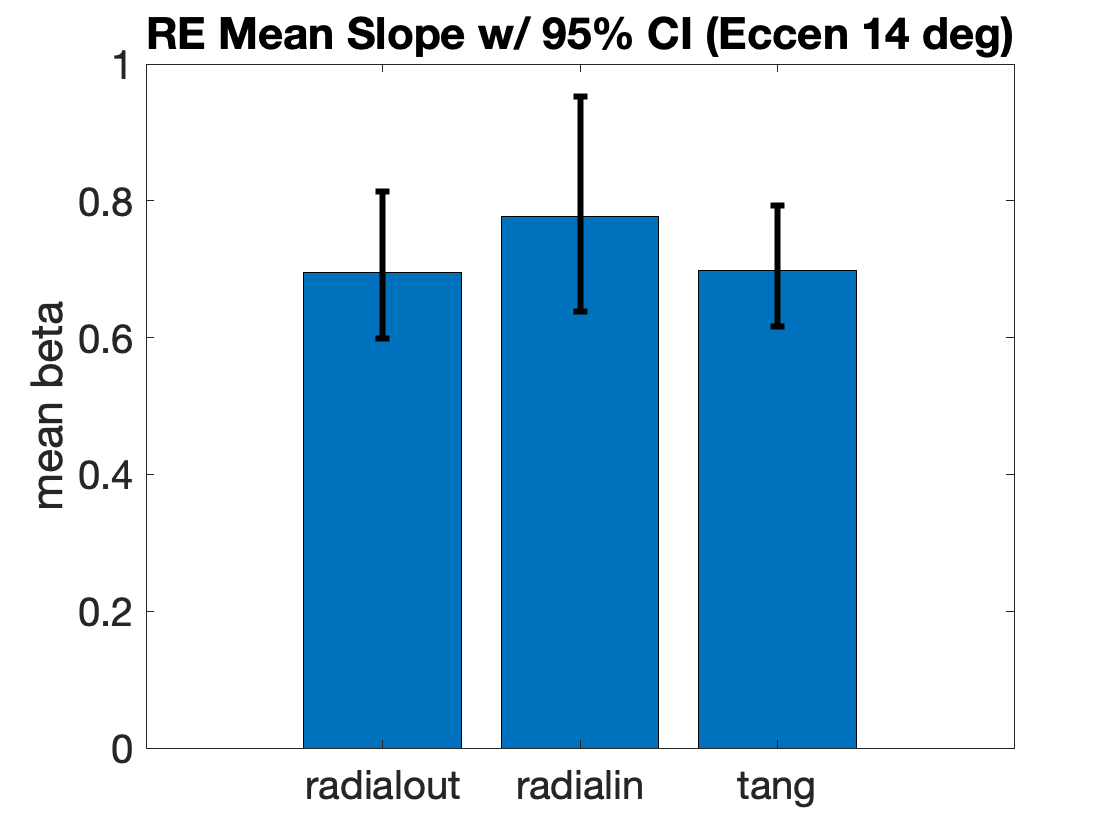
\includegraphics[scale=.2]{Images/MeanSlopeError_95ci_RE_eccen14.png}
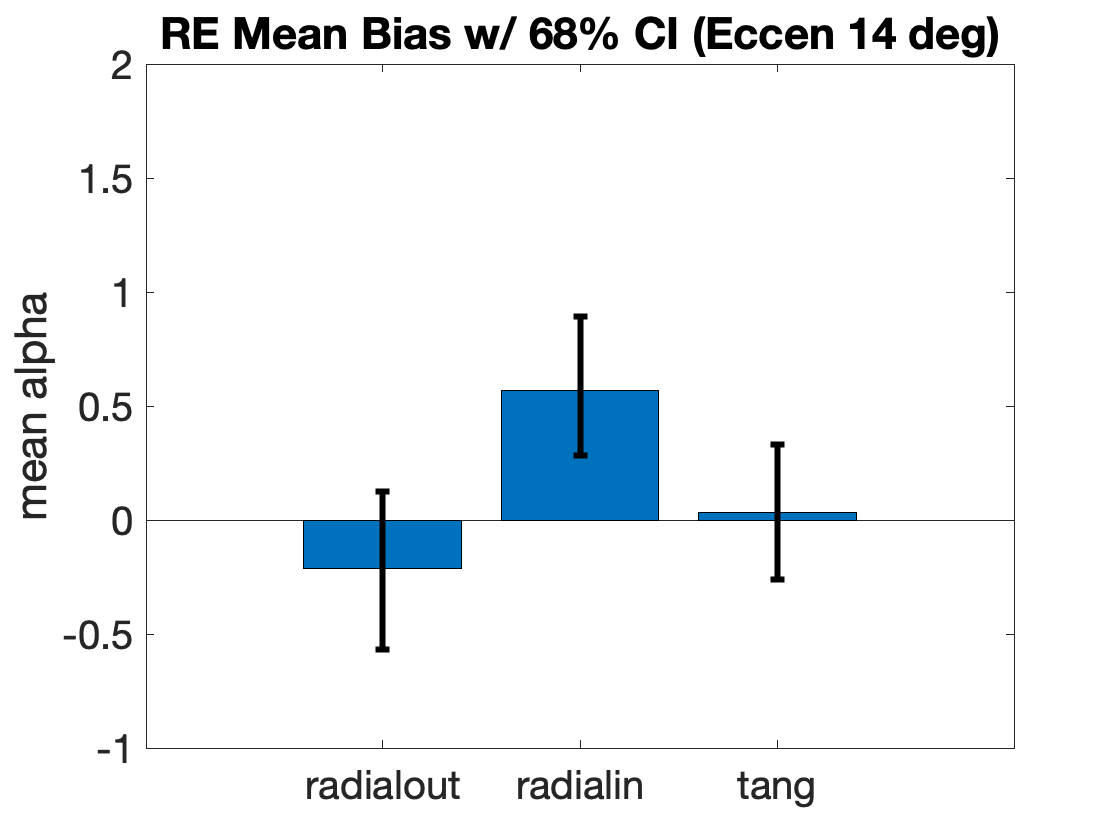
\includegraphics[scale=.2]{Images/MeanBiasError_68ci_RE_eccen14.png}
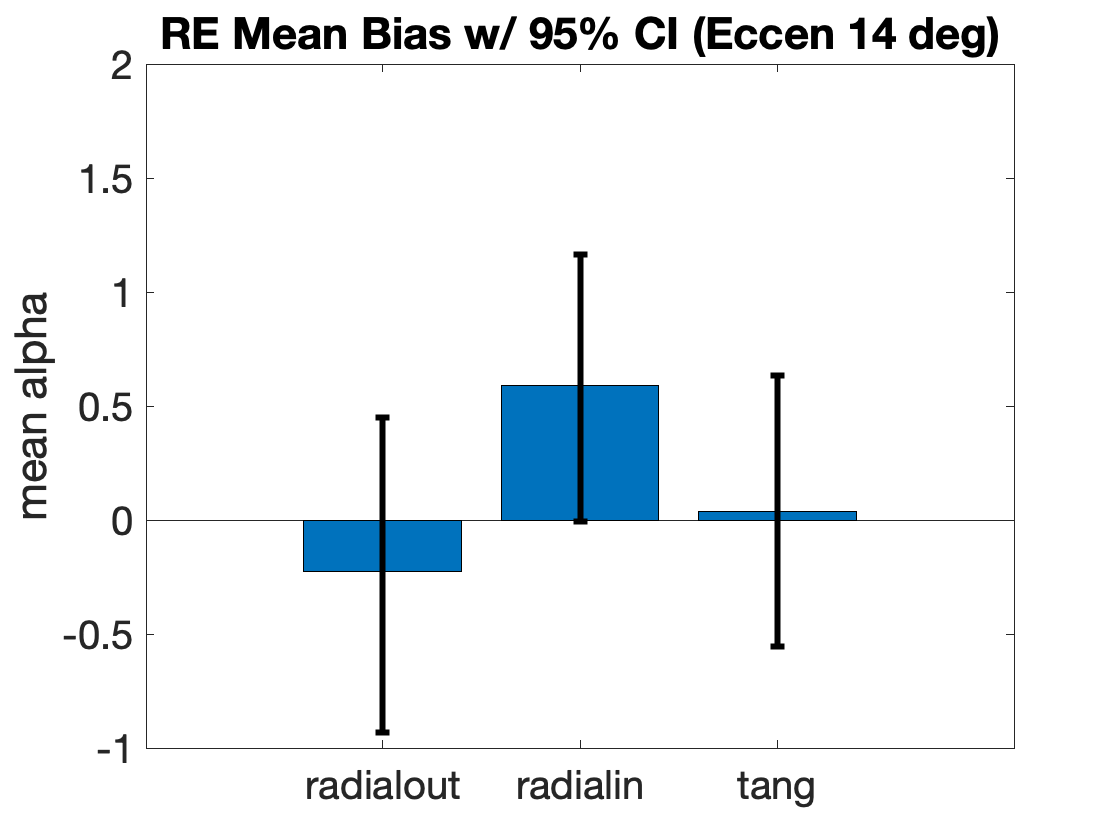
\includegraphics[scale=.2]{Images/MeanBiasError_95ci_RE_eccen14.png}
\caption{Top right/left: RE data (40 trails per angle -- new data).  Same layout as previous pages, but for double eccentricity (speed of 4 deg /s). Note: not all angles tested.}
\end{figure}

\newpage
\subsection{Current number of trials (RE only)}
N\_Trials is the total number of trials for a particular condition.
Ans\_clock is the percentage of the observer answering clockwise out of the N\_Trials for that condition.
\begin{table*}[htb]
  \label{tbl:stats-and-correlations}
  %\small\begin{tabularx}{\linewidth}{X*{15}{c}}
  \small\begin{tabular*}{\linewidth}{l@{\extracolsep{\fill}}*{18}{c}}
    \toprule
    & \multicolumn{4}{c}{\textbf{Radial outwards}}\\ \cmidrule(r){2-18}
    & {-4} & {-3} & {-2.5} & {-2} & {-1.5} & {-1.25} & {-1} & {-.75} & {-.5} & {.5} & {.75} & {1} & {1.25} & {1.5} & {2} & {2.5}& {3}& {4} \\ [0.5ex]
    N\_Trials:  &    40 &    40 &    40 &    40 &    40 &    40 &    40&   40 &   40 &    40&    40&    40&   40&    40&    40 & 40 & 40 & 40\\
    Ans\_clock:  &  .05 &  0 &    .13 &    .15 &    .18 &    .2 &    .28 &   .33 &    .4&    .63&    .55&    .53&    .63&    .63&    .68&    .83 & .95 & .95\\
    N\_Trials:  &    40 &    40 &    40 &    40 &    40 &    40 &    40&   40 &   40 &    40&    40&    40&   40&    40&    40 & 40 & 40 & 40\\
    Ans\_clock:  &  .05 &  .15 &    .18 &   .25 &    .3 &    .25 &   .25 &    .38&    .4&    .53&    .7&    .75&    .63&    .68&    .75 & .83 & .9 & .95\\
    \bottomrule
  %\end{tabularx}
  \end{tabular*}
\end{table*}

\begin{table*}[htb]
  \label{tbl:stats-and-correlations}
  %\small\begin{tabularx}{\linewidth}{X*{15}{c}}
  \small\begin{tabular*}{\linewidth}{l@{\extracolsep{\fill}}*{18}{c}}
    \toprule
    & \multicolumn{4}{c}{\textbf{Radial inwards}}\\ \cmidrule(r){2-18}
    & {-4} & {-3} & {-2.5} & {-2} & {-1.5} & {-1.25} & {-1} & {-.75} & {-.5} & {.5} & {.75} & {1} & {1.25} & {1.5} & {2} & {2.5}& {3}& {4} \\ [0.5ex]
    N\_Trials:  &    40 &    40 &    40 &    40 &    40 &    40 &    40&   40 &   40 &    40&    40&    40&   40&    40&    40 & 40 & 40 & 40\\
    Ans\_clock:  &  .03 &  .1 &    .08 &    .08 &    .2 &    .3 &    .35 &   .38 &    .33&    .65&    .58&    .7&    .6&    .73&    .8&    .88& .88 & .88\\
    N\_Trials:  &    40 &    40 &    40 &    40 &    40 &    40 &    40&   40 &   40 &    40&    40&    40&   40&    40&    40 & 40 & 40 & 40\\
    Ans\_clock:  &  .1 &  .08 &    .15 &    .28 &    .2 &    .13 &    .35 &   .15 &    .3&    .35&    .65&    .78&    .75&    .68&    .78&    .78& .68 & .98\\
    \bottomrule
  %\end{tabularx}
  \end{tabular*}
\end{table*}


\begin{table*}[htb]
  \label{tbl:stats-and-correlations}
  %\small\begin{tabularx}{\linewidth}{X*{15}{c}}
  \small\begin{tabular*}{\linewidth}{l@{\extracolsep{\fill}}*{18}{c}}
    \toprule
    & \multicolumn{4}{c}{\textbf{Tangential (combined)}}\\ \cmidrule(r){2-18}
    & {-4} & {-3} & {-2.5} & {-2} & {-1.5} & {-1.25} & {-1} & {-.75} & {-.5} & {.5} & {.75} & {1} & {1.25} & {1.5} & {2} & {2.5}& {3}& {4} \\ [0.5ex]
    N\_Trials:  &    40 &    40 &    40 &  40 &  40 &    40 &    40&   40 &   40 &    40&    40&    40&   40&    40&    40 & 40 & 40 & 40\\
    Ans\_clock:  &  .03 &  .18 &    .13 & .18 &  .28 &    .2 &    .33 &   .58 &    .48&    .53&    .63&    .5&    .68&    .58&    .75&   .88 & .78 & .88\\
    N\_Trials:  &    40 &    40 &    40 &  40 &  40 &    40 &    40&   40 &   40 &    40&    40&    40&   40&    40&    40 & 40 & 40 & 40\\
    Ans\_clock:  &  .05 &  .15 &    .23 & .2 &  .3 &    .25 &    .4 &   .43 &    .48&    .5&    .48&    .85&    .75&    .8&    .68&   .78 & .9 & .85\\
    \bottomrule
  %\end{tabularx}
  \end{tabular*}
\end{table*}

\newpage
\section{Updates} 
\begin{itemize}
\item Design Related
	\begin{itemize}
	\item \textbf{Implemented log spacing (0.5 - 8) for stimuli for whenever eye tracking is being run. For comparison updates (speed etc.) used same values.}
	\item \textbf{Now will start running trials using 4 polar angles per block (block 1 = diagonal (e.g. upper left), block 2 = cardinal (upper vertical), block 3 = diagonal (upper left), ect.)}
	\item \textbf{This will motivate subject to keep fixation at center, evenly distribute tang and radial throughout trial, while maintaining ONE internal reference.)}
	\item \textbf{Estimated total runs = 16 blocks per eccentricity (8 blocks with unique internal motion vector x 2)}
	\item \textbf{Estimated total trials = 3,200 trials per eccentricity (10 angles (+-5 angles) x 20 trials per block x 16 block)}
	\item \textbf{Estimated total time = 320 min, or 5.3 hours (20 min per block x 16 runs)}
	\end{itemize}
\item Analysis Related
	\begin{itemize}
	\item \textbf{Tested several other parameters (speed, eccentricity).}
	\end{itemize}
\item Other improvements
	\begin{itemize}
	\item \textbf{Began implementation of eye tracking in code (still in progress)}
	\end{itemize}
\item For discussion
	\begin{itemize}
	\item \textbf{Why not seeing an effect with greater eccentricity?}
		\begin{itemize}
			\item{Could be out the range of the radial bias}
			\item{Could be the corners of my monitor (maybe need to re-test in eye tracker room}
			\item{Need to ensure stimulus diameter is at 2.5 deg -- right now testing at home and distance not controlled by chin rest}
		\end{itemize}
	\item \textbf{Will use eye tracker L1 for testing and finalization, and then hallway eye tracker for data collection}
	\item \textbf{Significant learning effect reported from my data..}
	\item \textbf{Note: how to ensure motion direction (and not orientation) is used by subject to determine c or cc for all conditions?}
		\begin{itemize}
			\item{I suggest increasing speed and lowering contrast to make motion more pronounced and orientation less pronounced.}
			\item{Is 2.5 stimulus diameter optimal? Or should increase?}
		\end{itemize}
	\item \textbf{Note: Radial condition block requires 1 internal vector (crossing fixation) while tang requires translating internal vector position base on stimulus location}
		\begin{itemize}
			\item{Can we run experimental block with 1 location (radial-in vs. radial-out vs. tangential) on experienced observer?}
			\item{Use adaptation somehow?}
			\item{Can we test at different eccentricities, and if effect increases we can argue that the effect is not solely due to fixation aiding radial conditions? If anything we might expect that if effect was due to fixation aiding radial performance, the effect would decrease (or remain constant) with eccentricity?}
		\end{itemize}
	\end{itemize}
\end{itemize}

\section{To Do} 
\begin{itemize}
\item Feedback from Feb 17, 2021
	\begin{itemize}
	\item ?Add eye-tracking data to experimental design to (1) ensure fixation, and (2) potentially can also look at whether drift patterns enhance percept
	\item ?Test on 4 locations now (all diagonal?)
	\item Think more about testing differences statistically (e.g. see if a common slope fits better than 3 different models), maybe use AIC
	\end{itemize}
\item Other
	\begin{itemize}
	\item Split first half of radial in and out to rule out any perceptual learning (since num radial trials is greater than for tang)
	\item Look into any dynamic staircase methods
	\item Double check sigma of gaussian (and at what eccentricity contrast drops below 1 perc)
	\item Fix occasional crashing error
	\item Make beep lower freq to make "incorrect" sound more intuitive
	\end{itemize}
\end{itemize}

\section{Extra Figures}
\subsection{Psychometric Function (Cumulative normal)}
\begin{figure}[H]
\centering % centers the figure
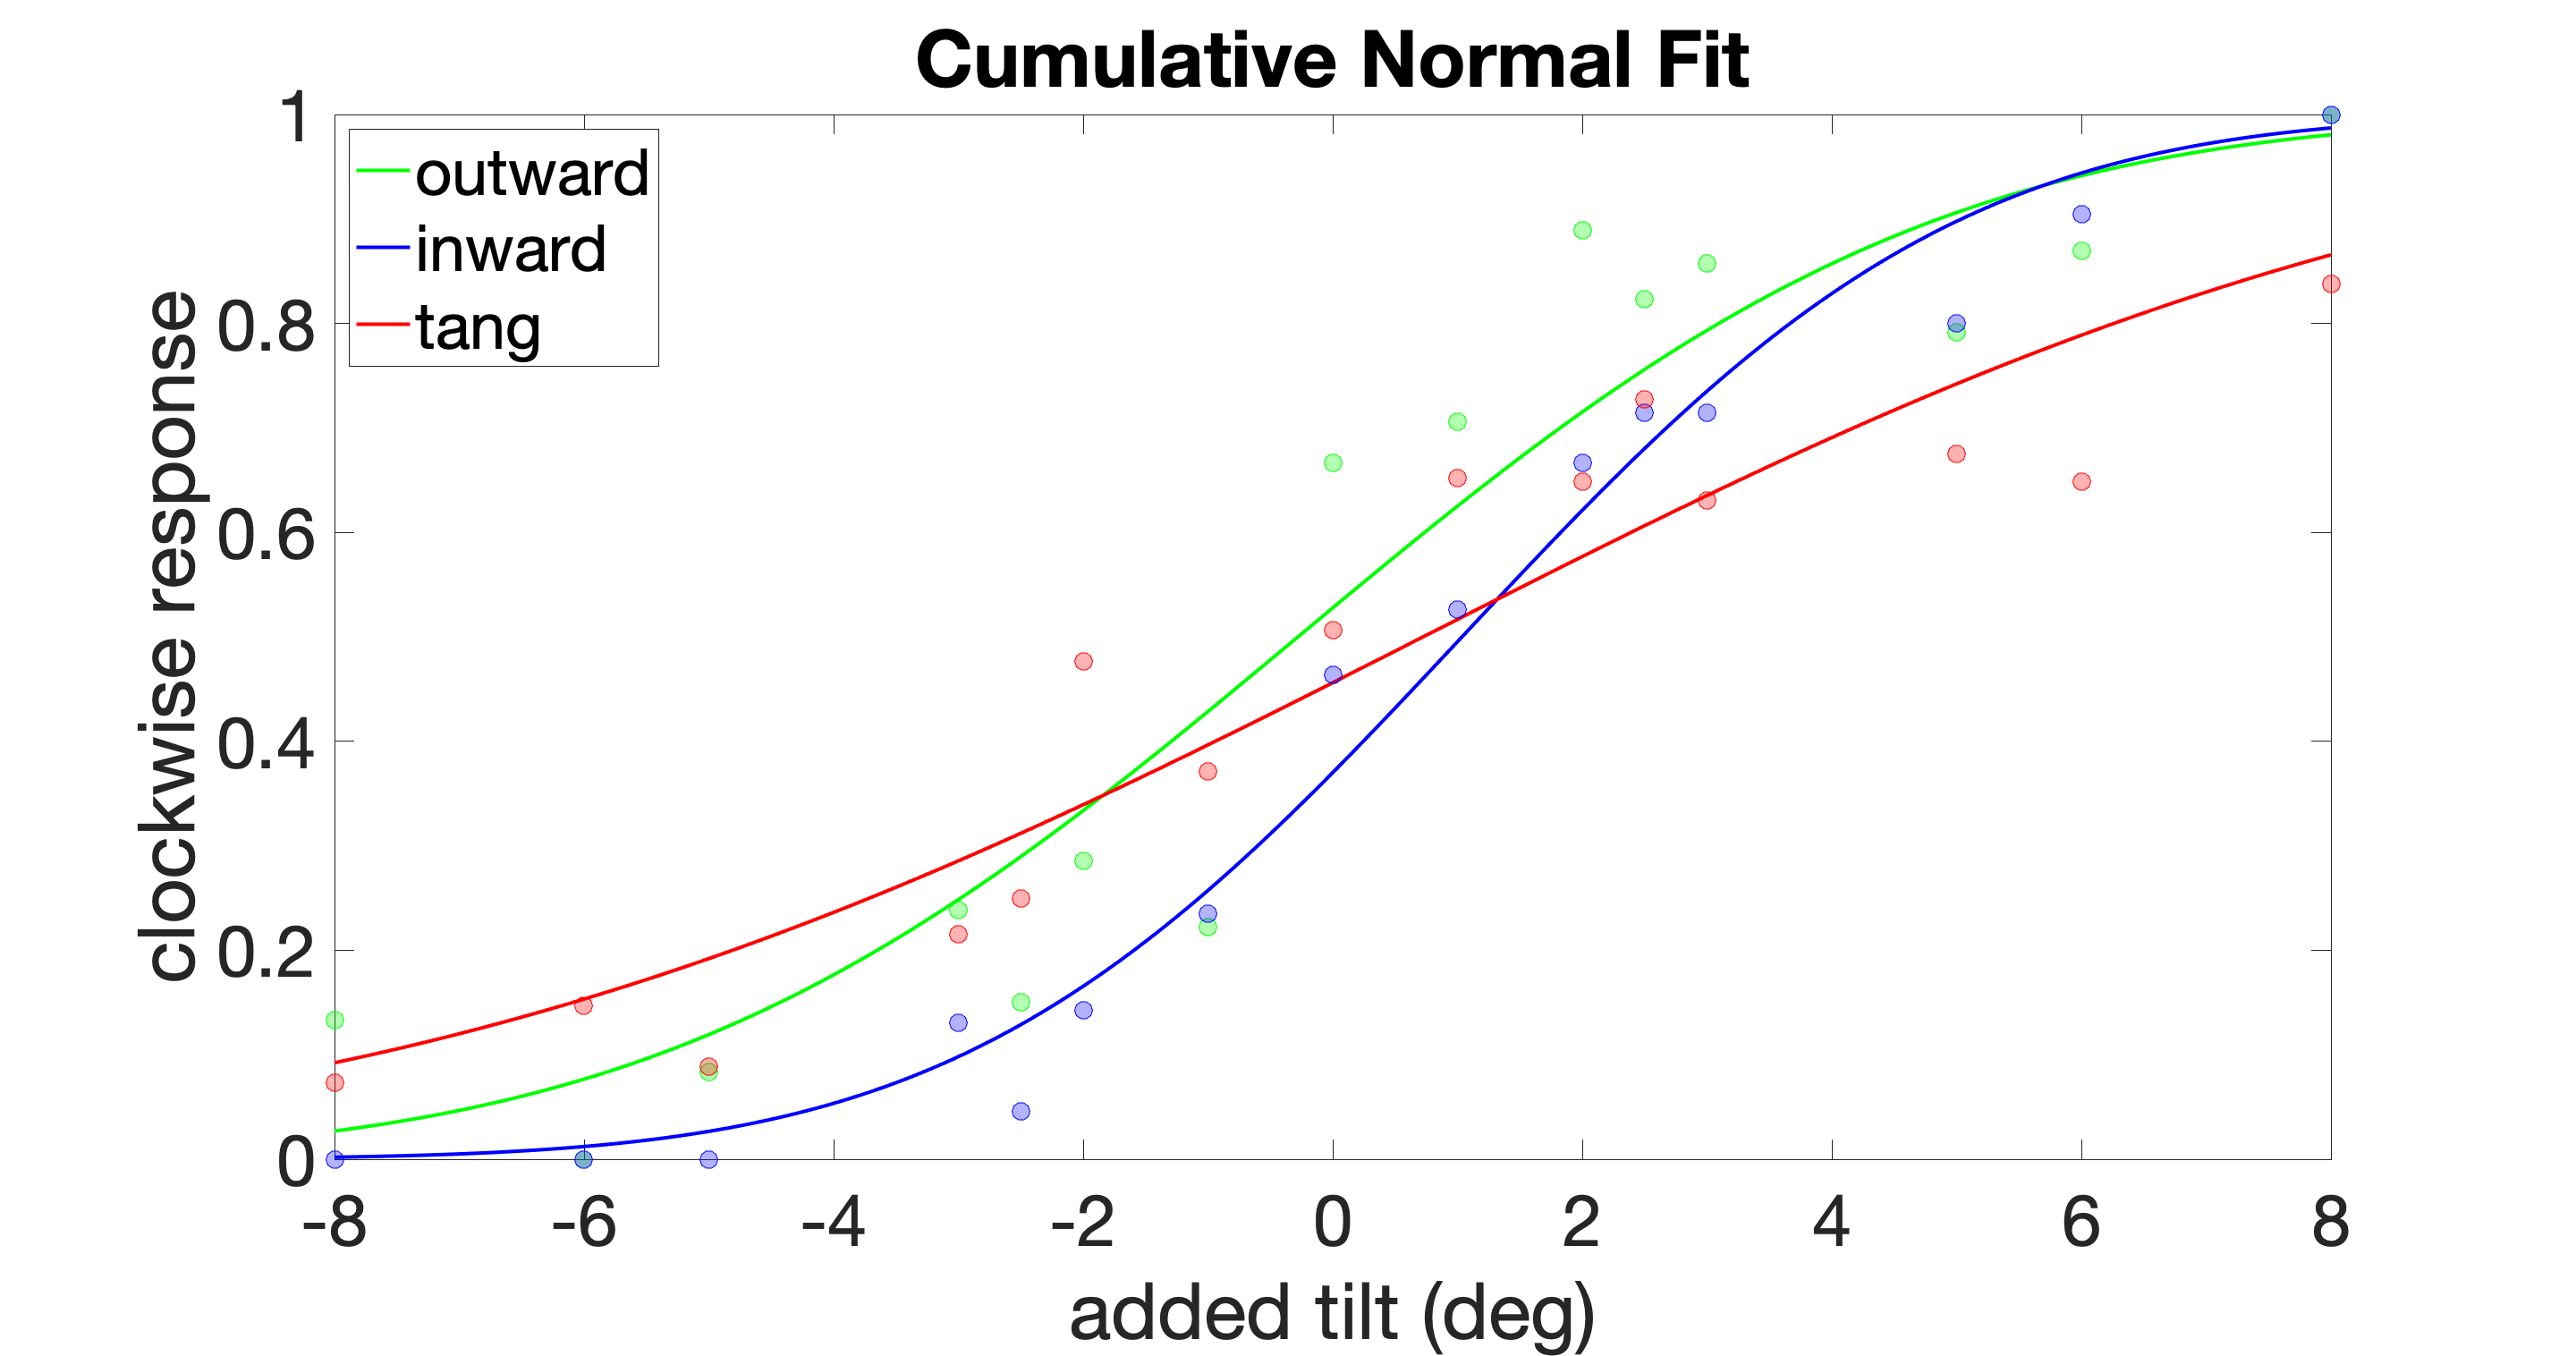
\includegraphics[scale=.08]{Images/PF_angles_old.png}
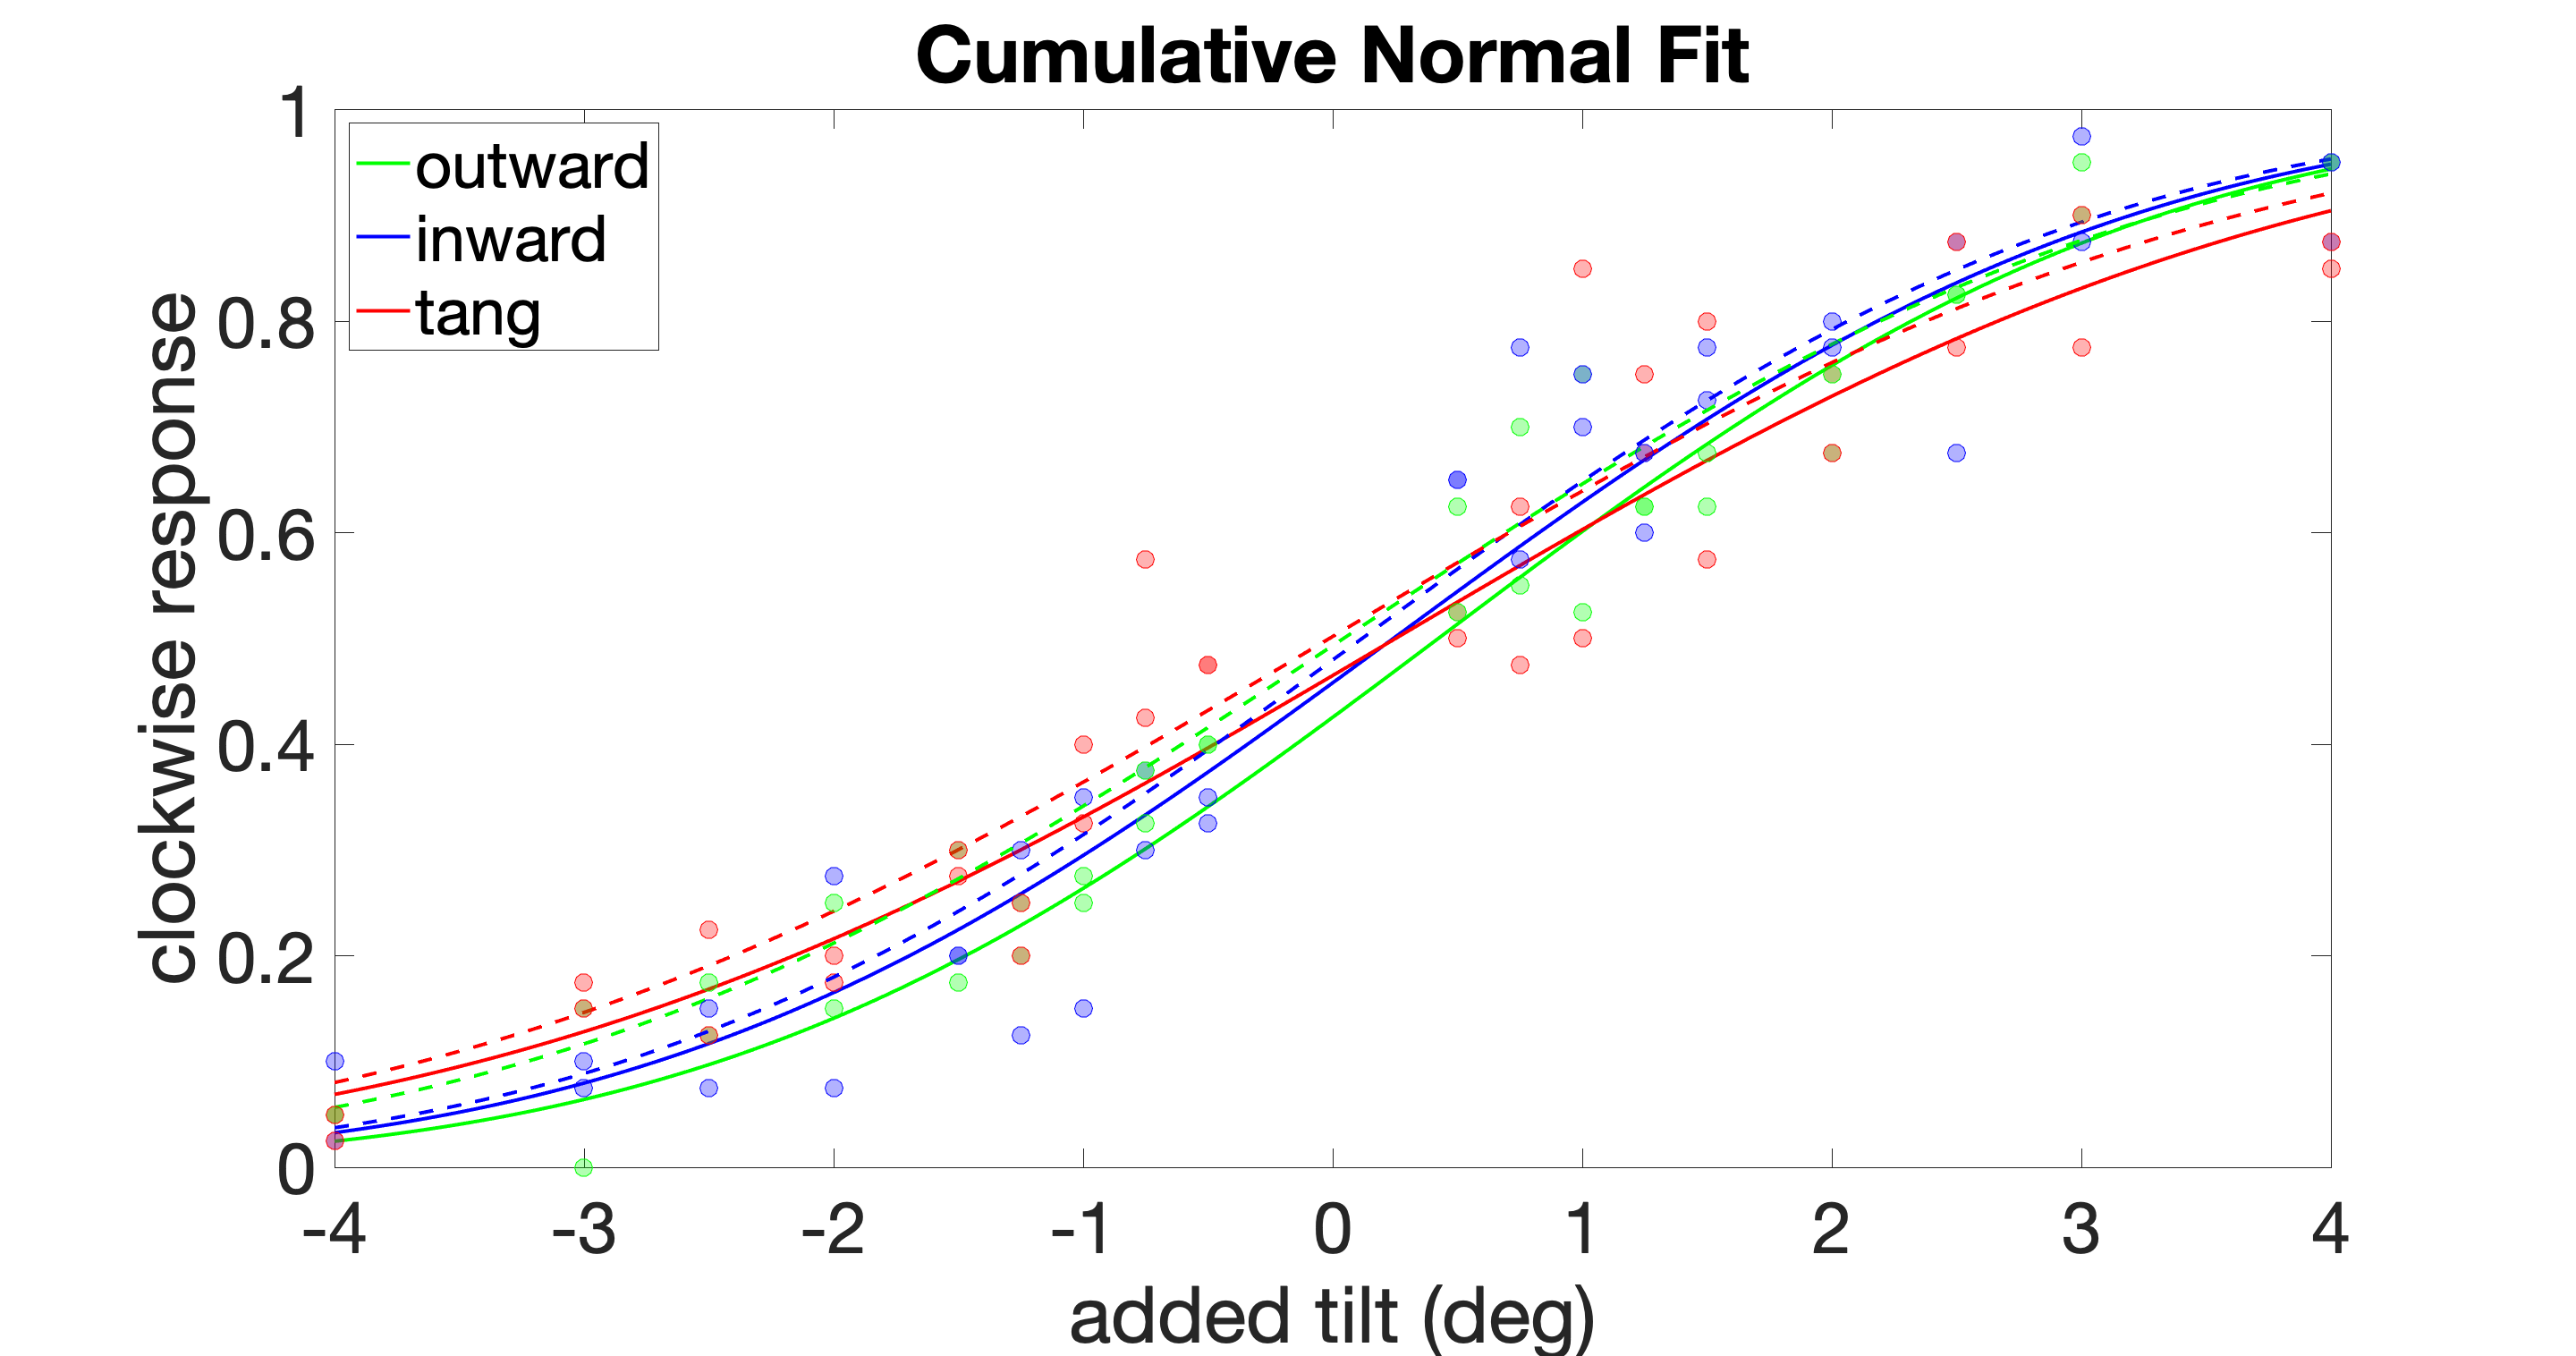
\includegraphics[scale=.08]{Images/PF_overlayed.png}
\caption{Left: previous RE data collected with blocks separated by radial-in, radial-out, tang-c, tang-cc. Right: newer RE data with blocks that contain same reference vector (e.g. blocks mixing radial-in/radial-out). This combines data across locations (40 trials per angle), and shows test (solid), re-test (dotted).}
\end{figure}

\section{Software to Cite}
\begin{itemize}
\item PsychToolbox Extensions (Brainard, 1997; Pelli, 1997; Kleiner et al, 2007)
\item Prins, N \& Kingdom, F. A. A. (2018) Applying the Model-Comparison Approach to Test Specific Research Hypotheses in Psychophysical Research Using the Palamedes Toolbox. Frontiers in Psychology, 9:1250. doi: 10.3389/fpsyg.2018.01250
\item Plummer, M. (2003, March). JAGS: A program for analysis of Bayesian graphical models using Gibbs sampling. In Proceedings of the 3rd international workshop on distributed statistical computing (Vol. 124, No. 125.10, pp. 1-10). (http://mcmc-jags.sourceforge.net/)
\end{itemize}

\end{document}